\documentclass{article}

\usepackage[T1]{fontenc}
\usepackage[utf8]{inputenc}
\usepackage{mdwlist} 
\usepackage{hyperref} 
\usepackage{float} 
\usepackage{listings} 
\usepackage[super]{nth} 
\usepackage{caption}
\usepackage{subcaption}
\usepackage[export]{adjustbox} 


\usepackage{graphicx} 
\graphicspath{ {images/} } 





\usepackage{hyperref}





































\begin{document}





\thispagestyle{empty}

\begin{figure}[H]
    
\includegraphics[width=0.5\textwidth, center]{ucd_logo_png}
\end{figure}

\vspace{3em}

\begin{center}
	{\LARGE \textbf{Recommender System For Tweets}} \\
	
	\vspace{0.5em}
	
	\textsl{Team $\lambda$ Lovelace -- Final Report} \\
	
	\vspace{1.5em}
	
	\textit{by} \\
	
	\vspace{1.5em}
	
	Xinqi Li \\
	Marc Laffan \\
	Junyang Ma \\
	Jón Rúnar Helgason \\
	Eazhilarasi Manivannan \\
\end{center}

\vspace{5em}

\begin{center}
    \textbf{University College Dublin -- Ireland} \\
    \textbf{School of Computer Science \& Informatics} \\
    \textbf{Course}: Computer Science, Negotiated Learning MSc \\
    \textbf{Module}: COMP47250 -- Team Software Project 2016 \\ 
    
    \vspace{1.5em}
    
    \textbf{Academic Supervisors}: \\
    Dr. Brian Mac Namee, Dr. Derek Greene, Dr. Georgiana Ifrim
\end{center}

\vspace{2.5em}

\begin{center}
    \nth{19} August 2016
\end{center}









\newpage







\pagenumbering{arabic} 

\begin{center}
    {\Large \textbf{Abstract}} \\
    \vspace{2em}
    \parbox{0.85\textwidth}
    {\textsl{
        A content based recommender system for Twitter tweets. The main goal of the $\lambda$ Lovelace system is to personalise the users' feed based on their interests to combat noise and information overload inherent in traditional chronologically ordered Twitter feeds. Subject preference is sourced from the user’s personal tweets, retweets, and likes. Additional feedback such as \textit{more/less} from \textit{author} or \textit{subject} was collected from our own prototype iOS Twitter client. Tweets were sourced from the Twitter REST API but subject to hefty rate limits. To work around rate limits Celery workers were constructed to collect and persist tweets slowly over time to a RethinkDB database. A Python Flask webservice backend serves the iOS app recommended tweets and collects the additional user feedback. The recommender system employs a two tier term frequency document approach. First a narrow net is cast to catch the highest quality tweets, then a wider more general net is cast on the remaining tweets to obtain a preference order on as many tweets as possible. Evaluation experiments showed promising results for users with narrow subject interests but evaluators were too few to draw firm conclusions.
    }} \\
    \vspace{2em}
    {\scriptsize $\lambda$ $\lambda$ $\lambda$}
\end{center}

\noindent This is a final report submitted to the School of Computer Science \& Informatics in partial fulfilment of the requirements for the degree of Masters of Science in Computer Science at University College Dublin.

The purpose of the final report is to give an overall picture of the chosen project, to present the solution proposed and to summarise the findings. The report is one of a few deliverables in the 30 ECTS credit module \textit{COMP47250 Team Software Project 2016}. The module spanned 14 weeks, starting on the \nth{16} of May and culminating in a final submission on the \nth{19} of August 2016.
\\\\
Another major deliverable was the main working source code repository:
\\\\
\url{https://github.com/jonrh/lambda-lovelace}
\\\\
At the time of writing it was private but the team hopes to make it public at a later date after sensitive material has been removed. For the final submission the working Git repository was mirrored on the \nth{19} of August to the below repository as that was the official submission area:
\\\\
\url{https://github.com/ucd-nlmsc-teamproject/LambdaLovelace-Team}
\\\\
The team tracked progress throughout the project at the following blog:
\\\\
\url{https://jonrh.github.io/lambda-lovelace/}


\clearpage





\tableofcontents
\clearpage













\section{Introduction} 
The theme for the 2016 final group project was \textit{The Future of News}. The premise for our project is the observation that people are experiencing an information overload in social media \cite{information_overload}. Decades ago news or content creators were few (print, television, radio) compared to today. Now everyone with a computer or a smartphone can be a content creator. We believe that the future of news is going to be filtering and delivering personalised content. We see our project, a recommender system for tweets, as a stepping stone in that direction, starting with Twitter.
\\\\
Keen readers may know that Twitter already employs their own recommender system for tweets so why did we attempt the same? In essence it came down to ``unlucky'' timing and search for the incorrect words. 

The final project took place during the summer of 2016 but teams started formulating project ideas in the spring semester. We conceived our idea in the beginning of March. Unknown to us at the time Twitter announced in a blog post \cite{twitter-opt-in} on the \nth{10} of February tweet recommendations were available as an opt-in feature in the official Twitter mobile app. On the \nth{17} of March Twitter started to silently roll out tweet recommendations as an opt-out feature. None of the team members noticed the change. It was not until in week two of our project (\nth{23} of May) when we started to dig deeper into the literature review that we learned that Twitter had in fact already implemented much of what we intended to build.

This experience set a bit of a bittersweet tone for the remainder of the project. On one hand we regretted not having done a more thorough research in the early project proposal stage yet on the other hand we felt exhilarated knowing we had the right kind of ideas since Twitter was already heading where we were headed. They just beat us to it.
\\\\
The name of our team, $\lambda$ Lovelace, is an homage to lambda calculus invented by Alonzo Church and Ada Lovelace, the first computer programmer.

\vspace{2em}

\begin{figure}[H]
    
\includegraphics[width=0.35\textwidth, center]{ll-logo}
    \caption{The logo for Team $\lambda$ Lovelace}
\end{figure}


\newpage





























\section{User Scenario: The Characters} 


Users of the $\lambda$ Lovelace system and the problems it solves.

\subsection{Target Users}
\begin{itemize*}
    \item Power users - this is an active Twitter user who follows more than 100 accounts. Their twitter home timeline is populated with approximately 200 tweets per day and they tweet, retweet or like approximately five times daily.
    \item Regular users - a user who is not very active and tweets roughly once a week. This user follows about 50 accounts.
    
    
\end{itemize*} 


\subsection{Why are they important?}
The system mainly targets power users, rather than the latter category. The power user has many tweets passing through their timeline every day and regularly engages in conversations on Twitter. These users compose a significant portion of the Twitter userbase, so it is important that they have the best possible experience when using Twitter. These users are also the most prone to the relevancy issue that plagues Twitter, which the $\lambda$ Lovelace system aims to combat.
As the recommender system's main focus is on filtering out the users home timeline of irrelevant tweets, the recommender system is most applicable to a power user. A regular user has a Twitter timeline where there is not enough activity to warrant a recommender system. They will see most of the news and tweets that they are interested in, along with irrelevant tweets. 

\subsection{What problem are you solving for them?}
The main issue that this project will solve arises when there is an overabundance of tweets. Indeed, Evan Williams (former Twitter CEO) stated in 2010 \cite{ceo}:

\begin{quote}
    \emph{\small "With 100 million tweets flowing through the system on a daily basis, there's something for everyone, but the real challenge is finding the most valuable stuff for you,"}  
\end{quote}

\noindent The following are two problem scenarios that twitter users currently face:

\begin{itemize*}
	 \item The users Twitter timeline showing irrelevant tweets.
	 \item The users relevant tweets being lost in the bulk of irrelevant tweets.
\end{itemize*}

\begin{figure}
    \centering
    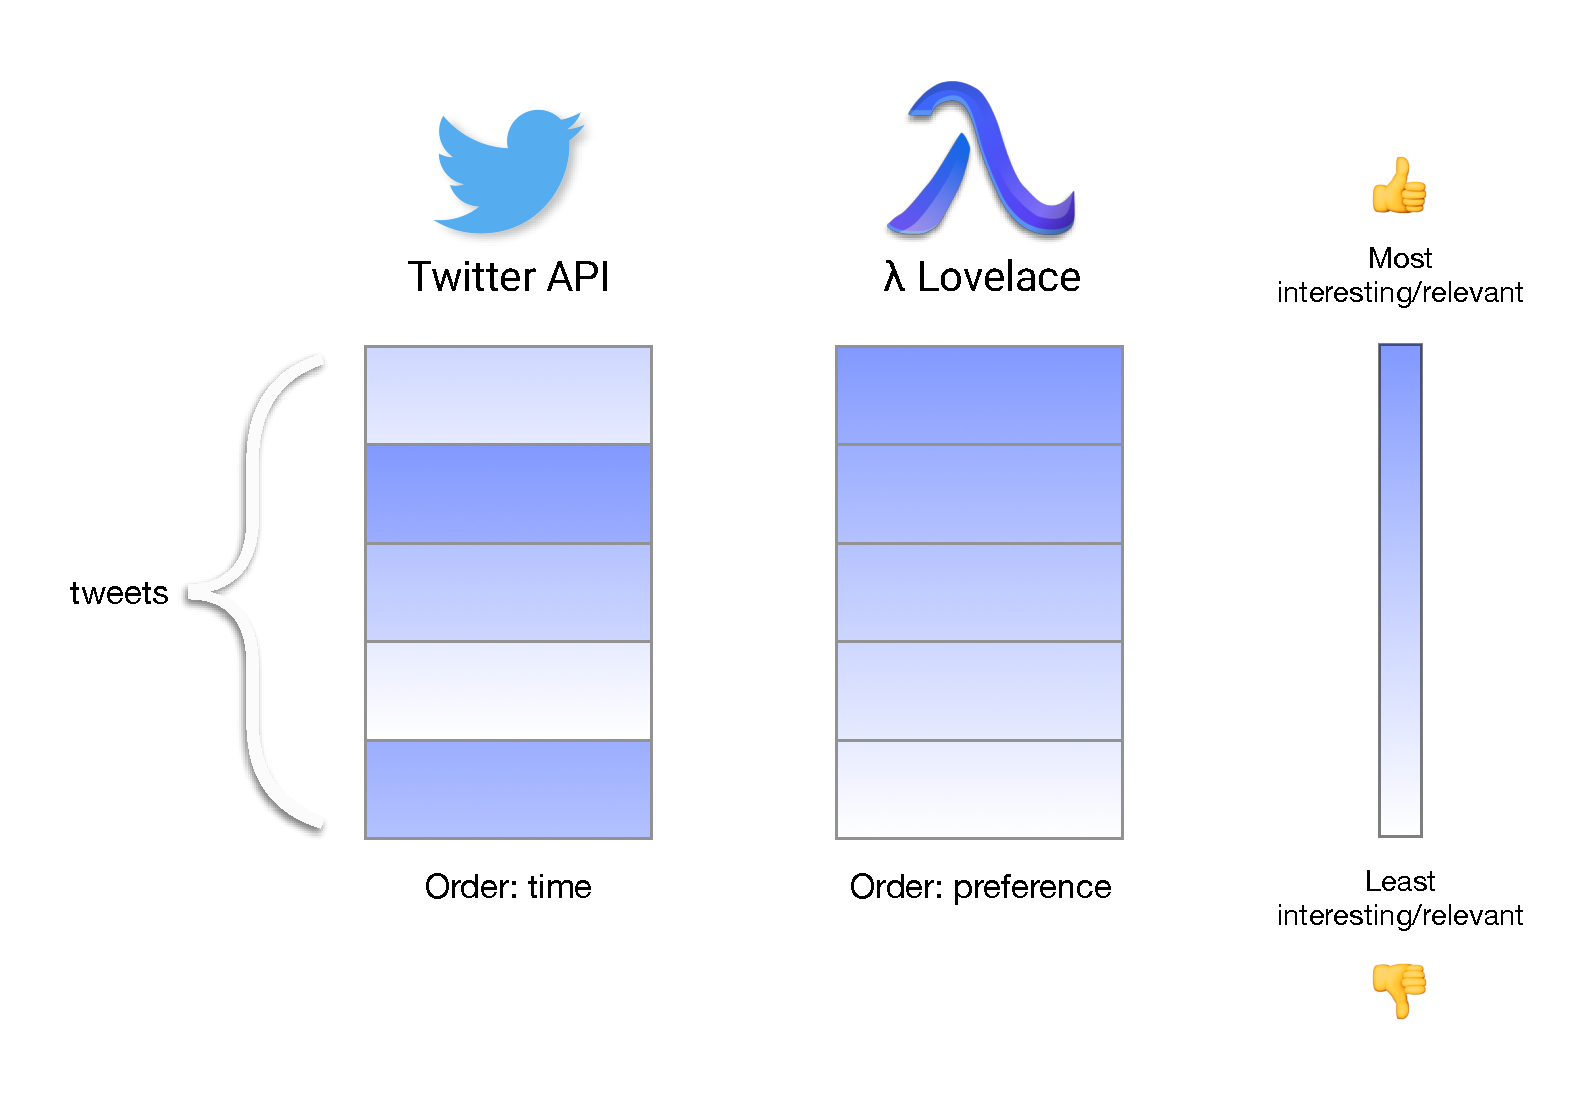
\includegraphics[width=0.95\textwidth]{explaining}
    \caption{The aim of the $\lambda$ Lovelace system. The Twitter API feed is ordered chronologically (newest first). Our aim is to create a feed where the most interesting/relevant tweets are shown first.}
\end{figure}

\subsubsection*{Problem One Scenario/Solution} 
In this scenario, there is an active twitter user "Robert" who works for a software development company using Microsoft Technology. He follows Scott Hanselman, a principal program manager from Microsoft, for interesting updates in Microsoft Technology. Scott Hanselman is also diabetic and posts tweets related to diabetes. Robert, who is not diabetic, may not be interested in Scott's diabetes related tweets. The recommender system will personalise Robert's timeline by prioritising relevant tweets, such as Scott Hanselmans technology related tweets, and filtering out his diabetes related tweets. 

\subsubsection*{Problem Two Scenario/Solution} 
Robert may follow many others who tweet on myriad topics. Due to the issues described in scenario one, the user must sift through many irrelevant tweets before reaching an occasional tweet that they are interested in. As the recommender system orders tweets by relevancy, there is far less of a chance that Robert will miss out on tweets in which he has a strong interest.


\newpage





































\section{Technical Problem} 

\subsection{Purpose} 
The $\lambda$ Lovelace project was created in order to tackle the issue of irrelevant tweets being shown in the timeline, and relevant tweets being overshadowed by irrelevant tweets. Twitter is not a segmented source of information and news, but comprises of people with a multitude of opinions from many diverse backgrounds. As a form of social media, its users are encouraged to give their opinions on current events, aspects of their background and their profession. Twitter itself stirs up discussion on current events with the use of hashtags, further promoting diverse conversations. All of this activity creates a very noisy environment, which makes it difficult for the user to access the tweets that are the most relevant to their interests. For example, the User Scenario section describes how Scott Hanselman discusses and promotes news on diabetes. His account also discusses his home life, children and other personal matters. This is likely due to the social media aspect of Twitter. 

However, the average user may not always be interested in reading tweets that are not directly related to their interests. For example, Andrew Clark recently tweeted the following\cite{clark1}:

\begin{figure}[H]
    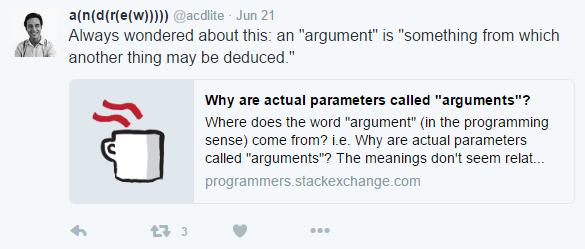
\includegraphics[width=0.6\textwidth, center]{clark1}
\end{figure}

Then shortly followed up with a political tweet, a subject completely unrelated to programming\cite{clark2}:

\begin{figure}[H]
    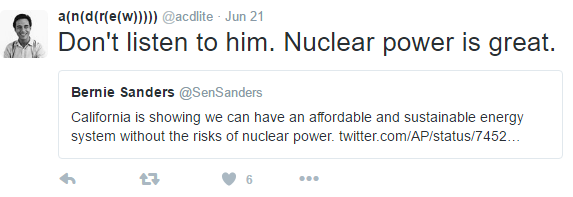
\includegraphics[width=0.6\textwidth, center]{clark2}
\end{figure}


\subsection{Core Technical Problem} 
The core technical problem for this project is recommending more relevant tweets to the user first, while demoting the least relevant tweets to appearing later. This is based entirely on the user's own interests on Twitter. The Andrew Clark tweets shown above are an example of how divided a Twitter account's content can be. Only software developers, or those with an interest in technology, should see the former tweet.
In order to create a system that provides such recommendations, this project must use the Twitter REST API \cite{twitter-rest-api}. However, there are rate limits placed on how many tweets can be extracted from the REST API at a time. Specifically, a user of the REST API may make 180 requests for a maximum of 3200 tweets every fifteen minutes for the user timeline. For the home timeline, a user of the API may only make fifteen requests for a maximum of 800 tweets every fifteen minutes. 

\begin{figure}[H]
    \centering
    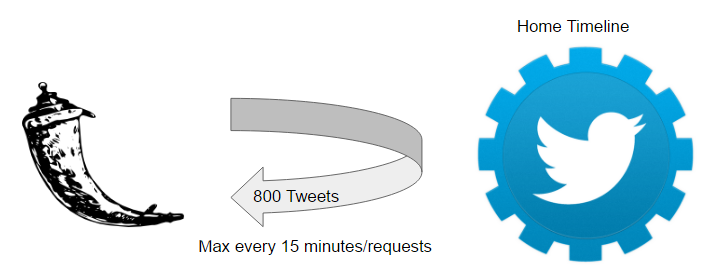
\includegraphics[width=0.6\textwidth]{rate_limit_1}
    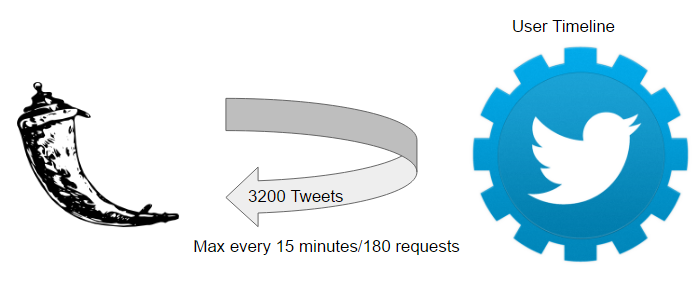
\includegraphics[width=0.6\textwidth]{rate_limit_2}
    \caption{Rate limits for the home timeline and user timeline}
    \label{fig:my_label}
\end{figure}


The issue of providing good quality recommendations was another problem that required work, as the system as a whole could be deemed lacklustre if the recommended tweets were not of value to the user. 



\subsection{Competitors} 


\subsubsection*{The Official Twitter mobile app}

\begin{figure}[H]
    
\includegraphics[width=0.35\textwidth, center]{twitter_logo}
\end{figure}
This app is the official mobile offering from Twitter for their system, which includes recommendations. This was discovered by the team in week two. It is seemingly allowed to access the Twitter API without the same restrictions as third-party apps. This app also has access to a set of personalised recommendations, which it is assumed comes from the API. Bearing all of this in mind, the Official Twitter mobile app is currently this project's main competitor. 


\subsubsection*{Flipboard}

\begin{figure}[H]
    
\includegraphics[width=0.35\textwidth, center]{flipboard_logo}
\end{figure}

Flipboard is a social news aggregator that provides personalised news article recommendations to the user, but is not a direct competitor to $\lambda$ Lovelace as it is not solely reliant on twitter for its content. It does however, still provide personalised recommendations on the iOS platform, albeit mainly for news articles. Flipboard provides a novel solution to the cold-start problem by suggesting a broad topic preference to the user when they first log in. When selected, these topics  are in-turn used to suggest more narrow-focused aspects of that topic as a new topic. This process allows Flipboard to eventually narrow down the users interests to very specific aspects of a broad subject. For example, research for this app has shown that it is possible to narrow down from the broad category of “technology”, to the more specific term “agile development” upon initial setup of the app. Once the app was running, it shortly suggested “JavaScript”.

\subsubsection*{News360}

\begin{figure}[H]
    
\includegraphics[width=0.35\textwidth, center]{news360_logo}
\end{figure}

News360 is another social news aggregator, very similar to Flipboard that also focuses on news articles from large publishers. However, where Flipboard asks for general topics to indicate preference,  News360 requires users to vote with a thumbs up/down option. This is somewhat similar to $\lambda$ Lovelace's like/dislike functionality for tweets. News360 also provides summaries of their articles, although this summarisation of news does not apply to the $\lambda$ Lovelace project. Its cold-start solution also allows users to “love” topics, as well as like them. This allows for further emphasis on topics that strongly interest the user.


\newpage
















































\section{Technical Solution} 

\subsection{What does the system do?} 

The system consists of an iOS client for the front-end and a Flask\cite{flask} web server for the back-end, which houses a recommender system. Upon logging in, the iOS client displays the filtered user's tweets. This filtering is performed by the recommender system. Uninteresting or irrelevant tweets are deferred while interesting tweets are prioritised for primary visibility. Rollbar is used to report errors in production, while Jenkins provides continuous deployment and RethinkDB is used to store tweets. Celery is used to automate the task of storing tweets in the database.




\subsection{How does it work?} 

\begin{figure}[H] 
    \centering
    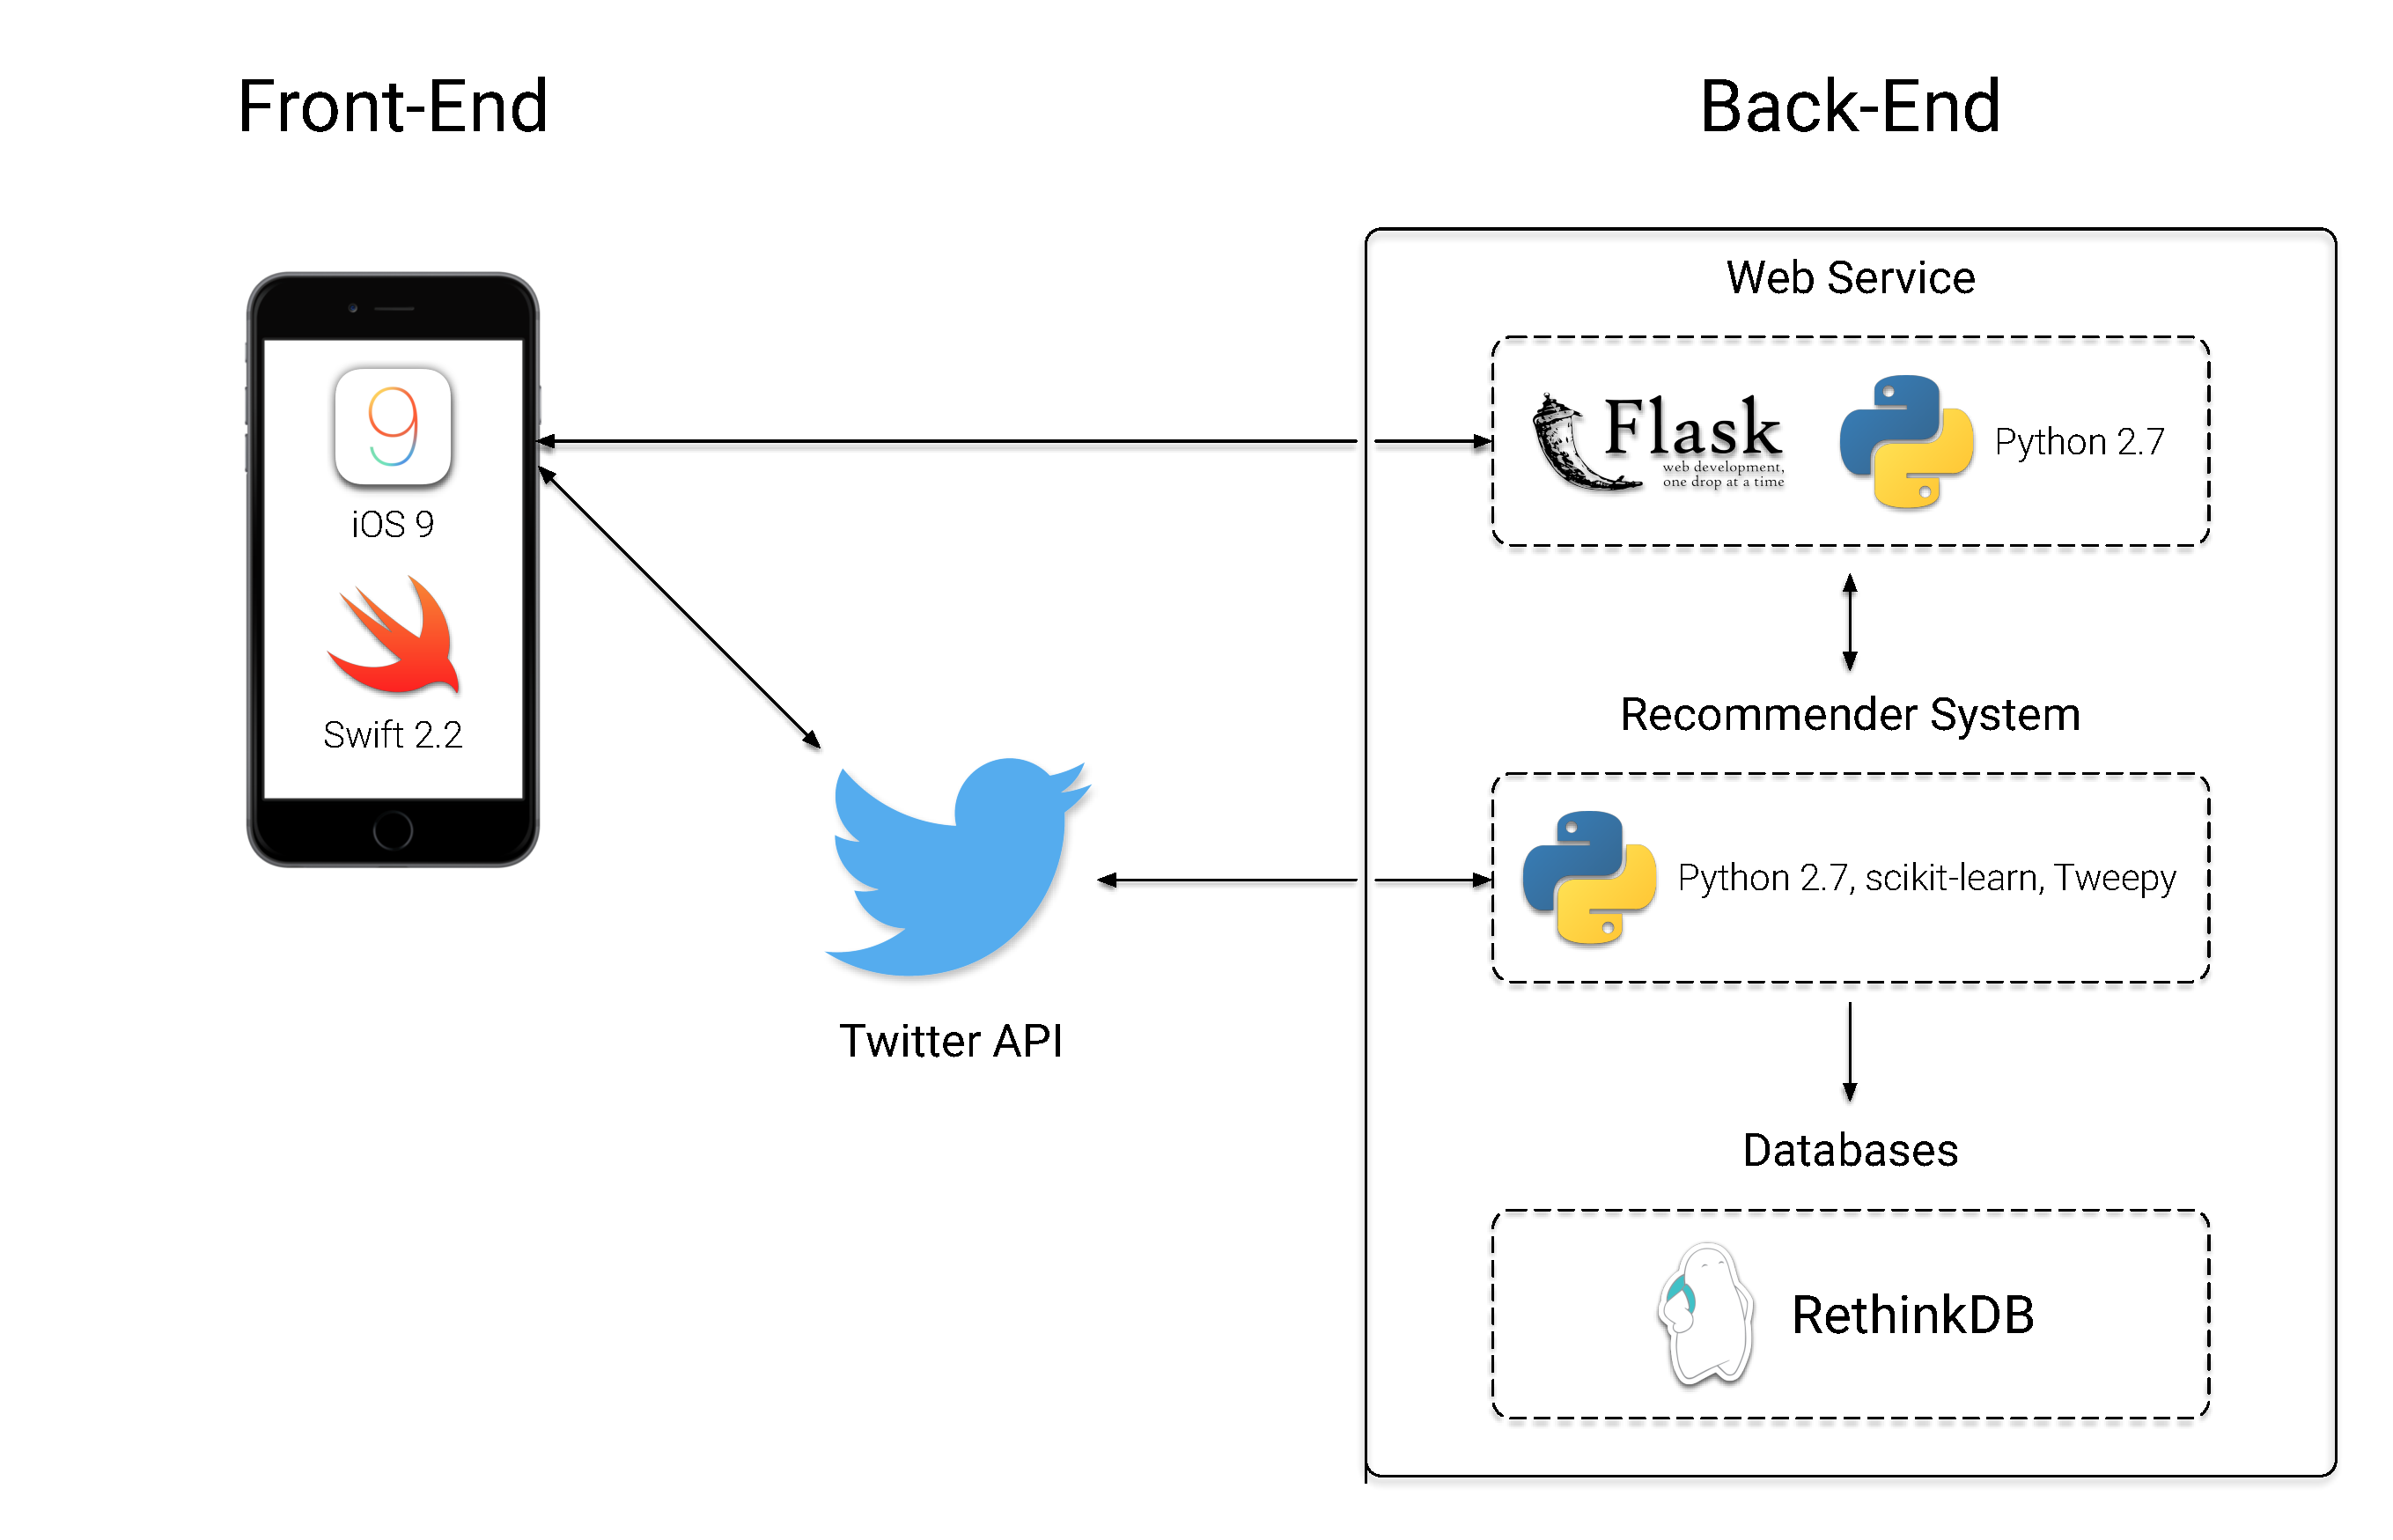
\includegraphics[width=\textwidth]{system_overview}  
    \caption{System Overview}
\end{figure}

First, the user must give the app permission to access their Twitter data. After that, the iOS client makes a request to the server. When the server first receives an iOS API request, it gets the users access token which enables the server to make authorised calls to the Twitter API. The server then uses this token to communicate with the Twitter API and fetch the users data. Following this, the raw data is stored in the database and sent to the recommender system to generate recommendations. 
Lastly, the server will return the generated recommendations from the recommender system to the iOS client so that the user can see their personalised tweet feed. The coloured dots on the left of the users screen indicate the relevance of tweets based on the user's interests.


\subsection{Front-End} 

The Swift programming language was chosen to develop the iOS client due to the teams familiarity with the language and the lack of Twitter app on the platform. The iOS client currently implements the following functions: \hyperlink{oauth}{OAuth login}, communication with the Flask API, author/tweet feedback, and Tweet data presentation.

\subsubsection*{OAuth login} 

Because Twitter's REST API requires each request to be authorised, the system needs the users login details for their Twitter account to grant it access to the users Twitter data. OAuth login is a complex process, so the third party library OAuthSwift \cite{oauthswift} was chosen to handle the users login function. It only requires the system to configure a few parameters, such as \textit{consumerKey} and \textit{consumerSecret}. OAuthSwift then performs the login process, opening Twitter's website and sending a request to the Twitter authorisation API. Lastly, it returns the OAuth access token which is then stored on the iOS client to avoid requiring repeated logins when using the app.

\subsubsection*{Communication with Flask} 
Alamofire \cite{alamofire} is a popular Swift library which provides an elegant and concise way to handle HTTP network requests. The system uses it to compose dynamic HTTP requests and to append the OAuth access token to URLs. It is also used to decode JSON responses returned from the Flask server.

\subsubsection*{Tweet data presentation} 
After the raw JSON data is received, it needs to be converted from JSON data to a Swift primary object, like a list or dictionary. The SwiftyJSON \cite{swiftyjson} library is used to accomplish this. Then, the tweet list is hooked up to an iOS \textit{UITableView} which is a powerful iOS UI component that is suitable for displaying a list with data. The Flask server also sends weight values for each tweet, which is calculated by the recommender system to represent how much the user may like a tweet. The iOS client calculates the colour hue for the the associated weight value, which is used to set the background colour of the dot to the left of each tweet.


\newpage


\begin{figure}[H]
    \centering
    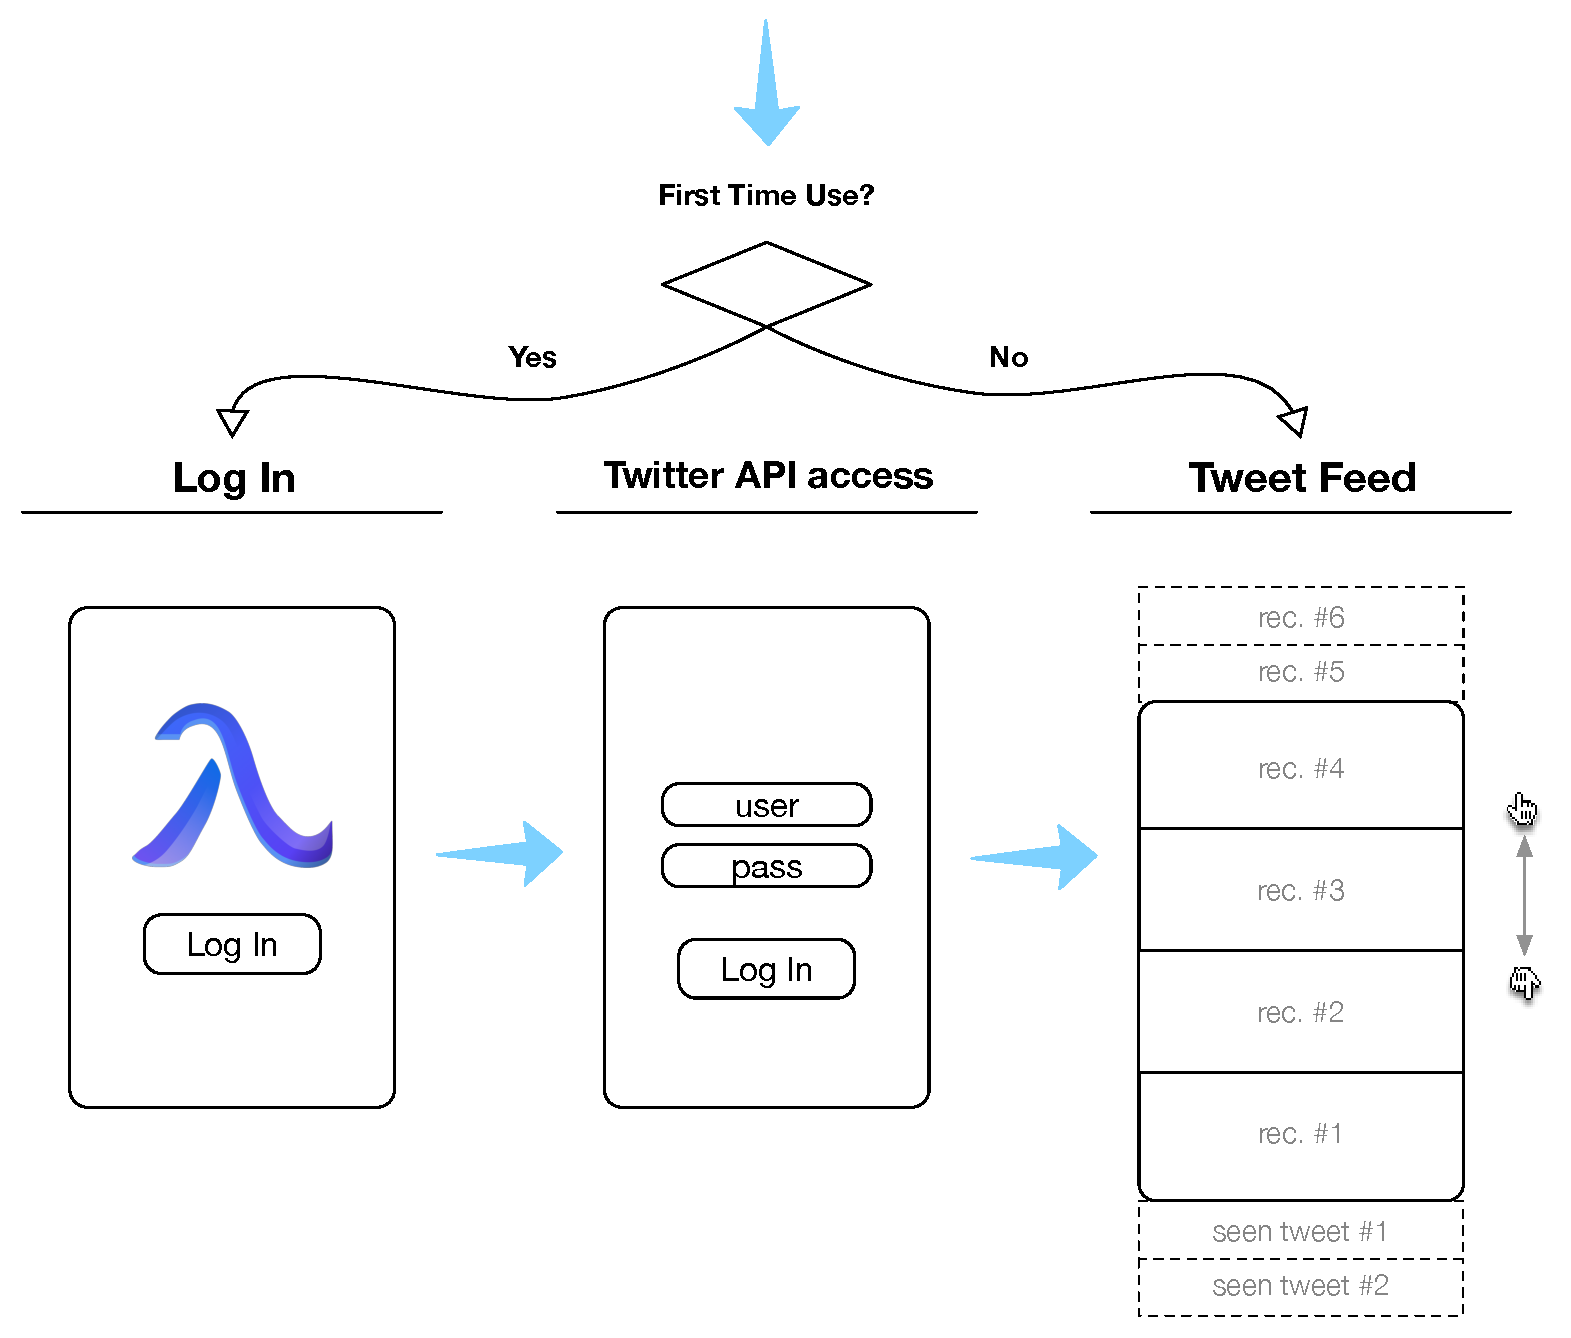
\includegraphics[width=0.78\textwidth]{ios_wireframe_1}  
    \caption{Wireframe of the flow in the iOS app}
\end{figure}

\begin{figure}[H]
    \centering
    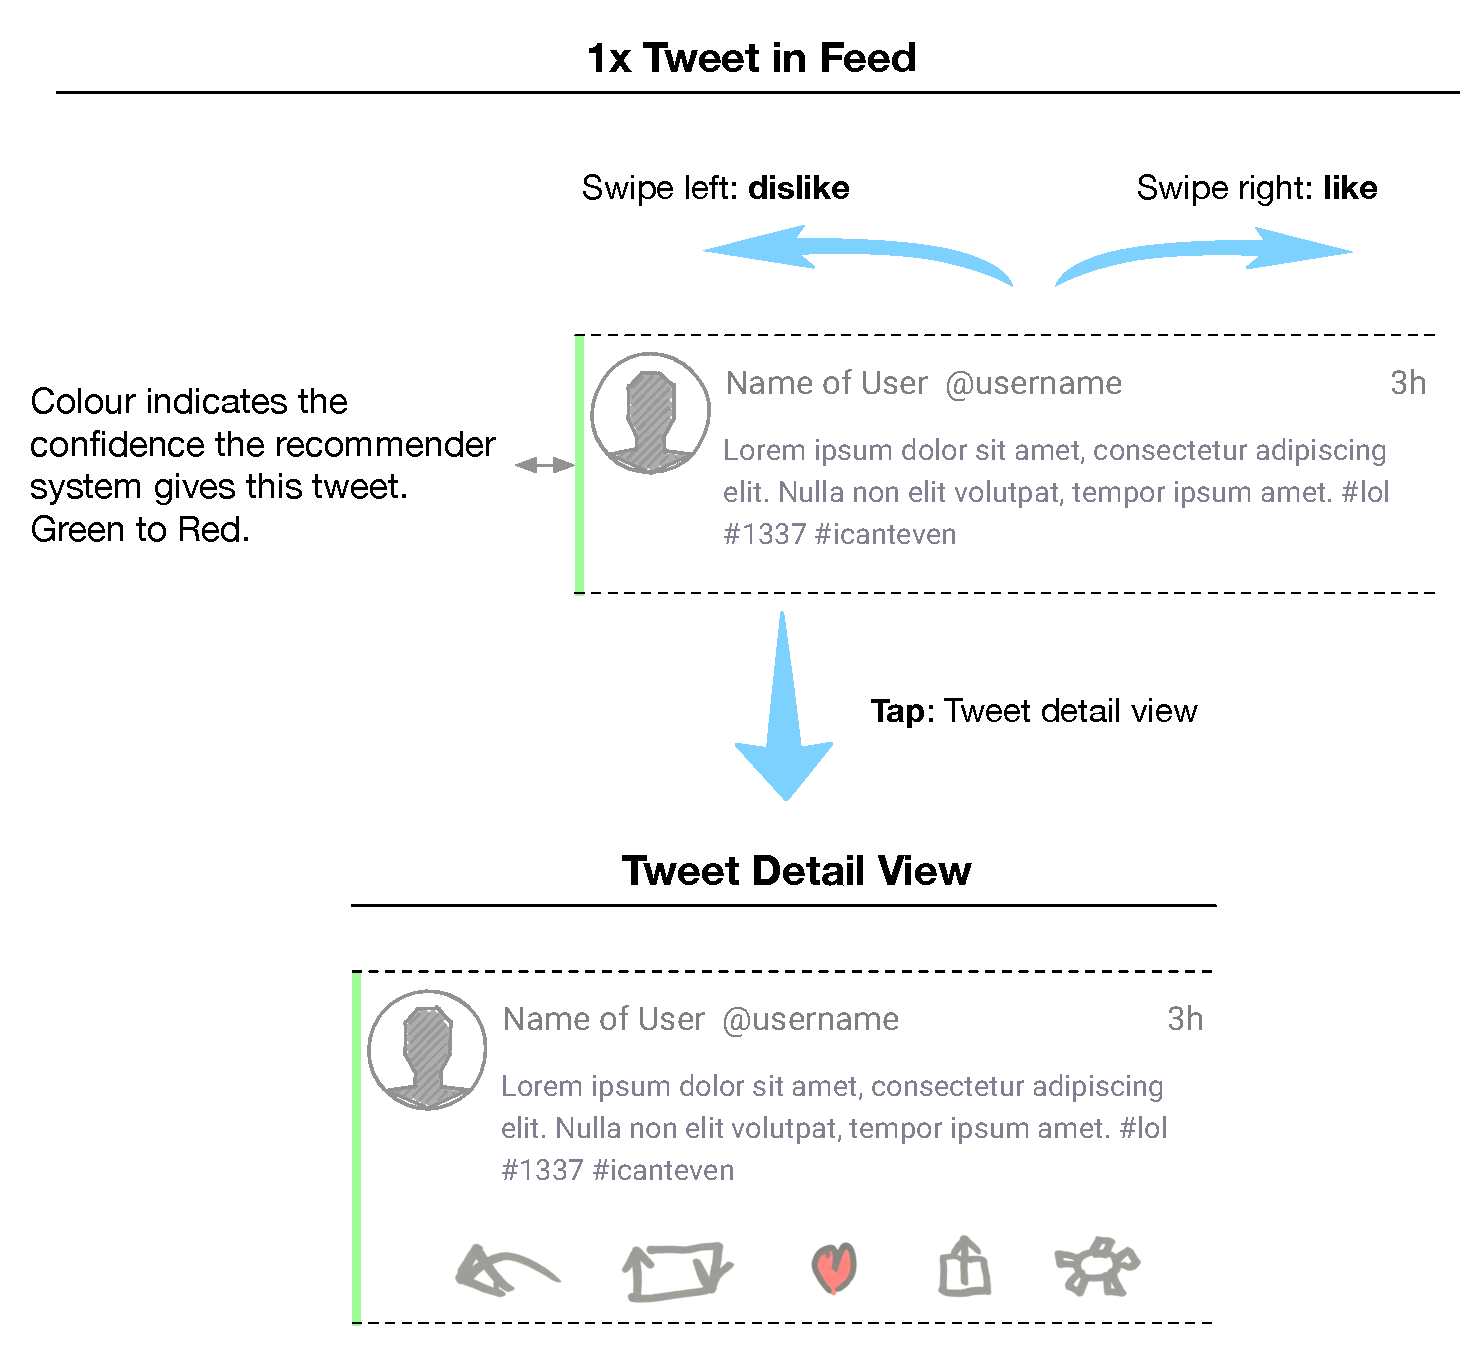
\includegraphics[width=0.78\textwidth]{ios_wireframe_2}  
    \caption{Wireframe of a Tweet in feed and detail view}
\end{figure}


\newpage


\begin{figure}[H]
    \centering
    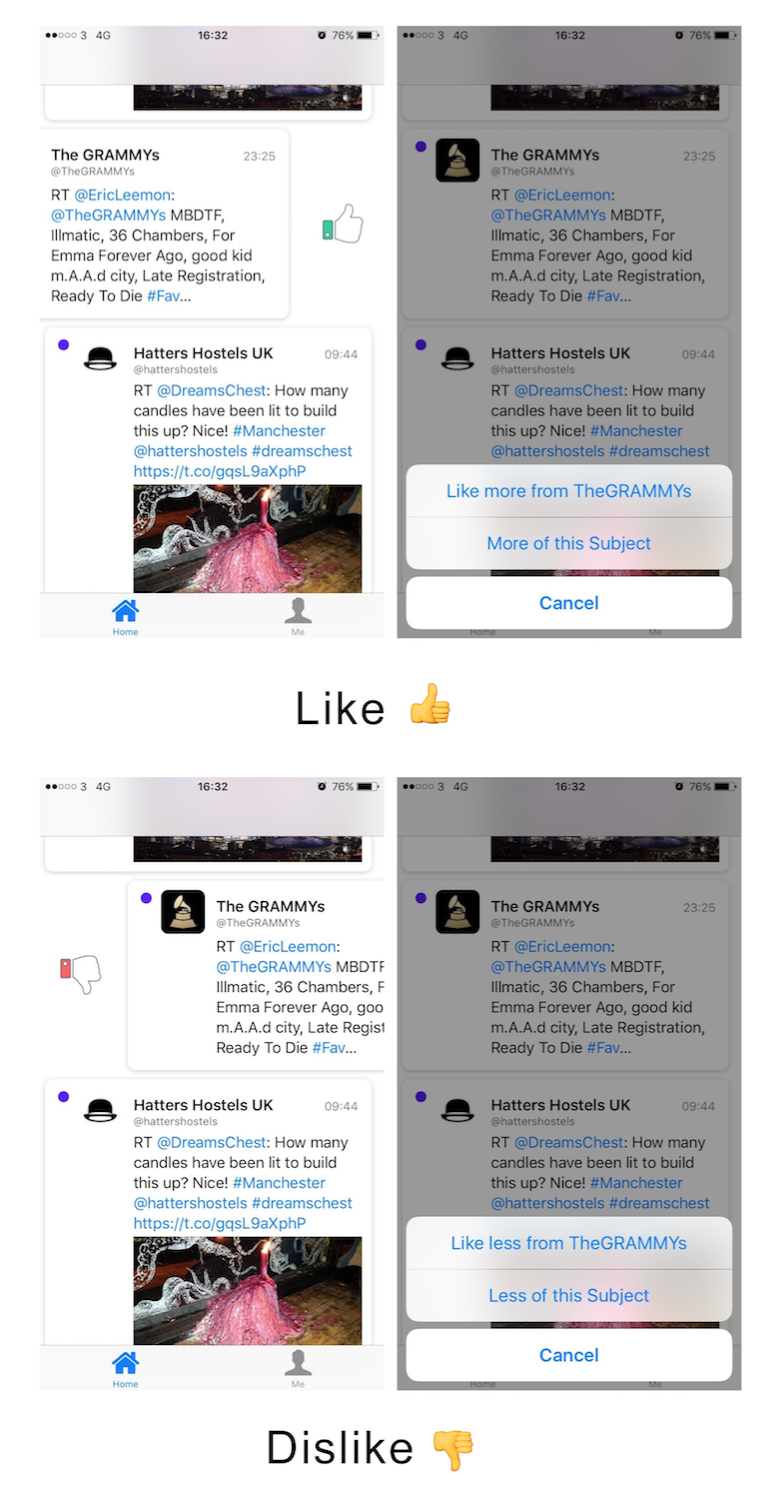
\includegraphics[width=0.6\textwidth]{like_dislike}  
    \caption{Screenshots of Like/dislike function}
\end{figure}

A user can choose either like/dislike on a single tweet along with a reasons. These events will be recorded and used to optimise the recommender system for that user.


\newpage



\subsection{Back-End} 

Our back-end consists of the following: Flask web server, RethinkDB database, Celery, Jenkins, Rollbar and our recommender system. Originally Python 3.5 was used but due to compatibility issues between libraries we downgraded to Python 2.7.



\subsubsection*{Docker} 
To standardise deployments we maintained a single Docker image with Ubuntu 14.04, Python 2.7, third party libraries and our source code. This image was used to run 4 separate containers:

\begin{figure}[H]
    \centering
    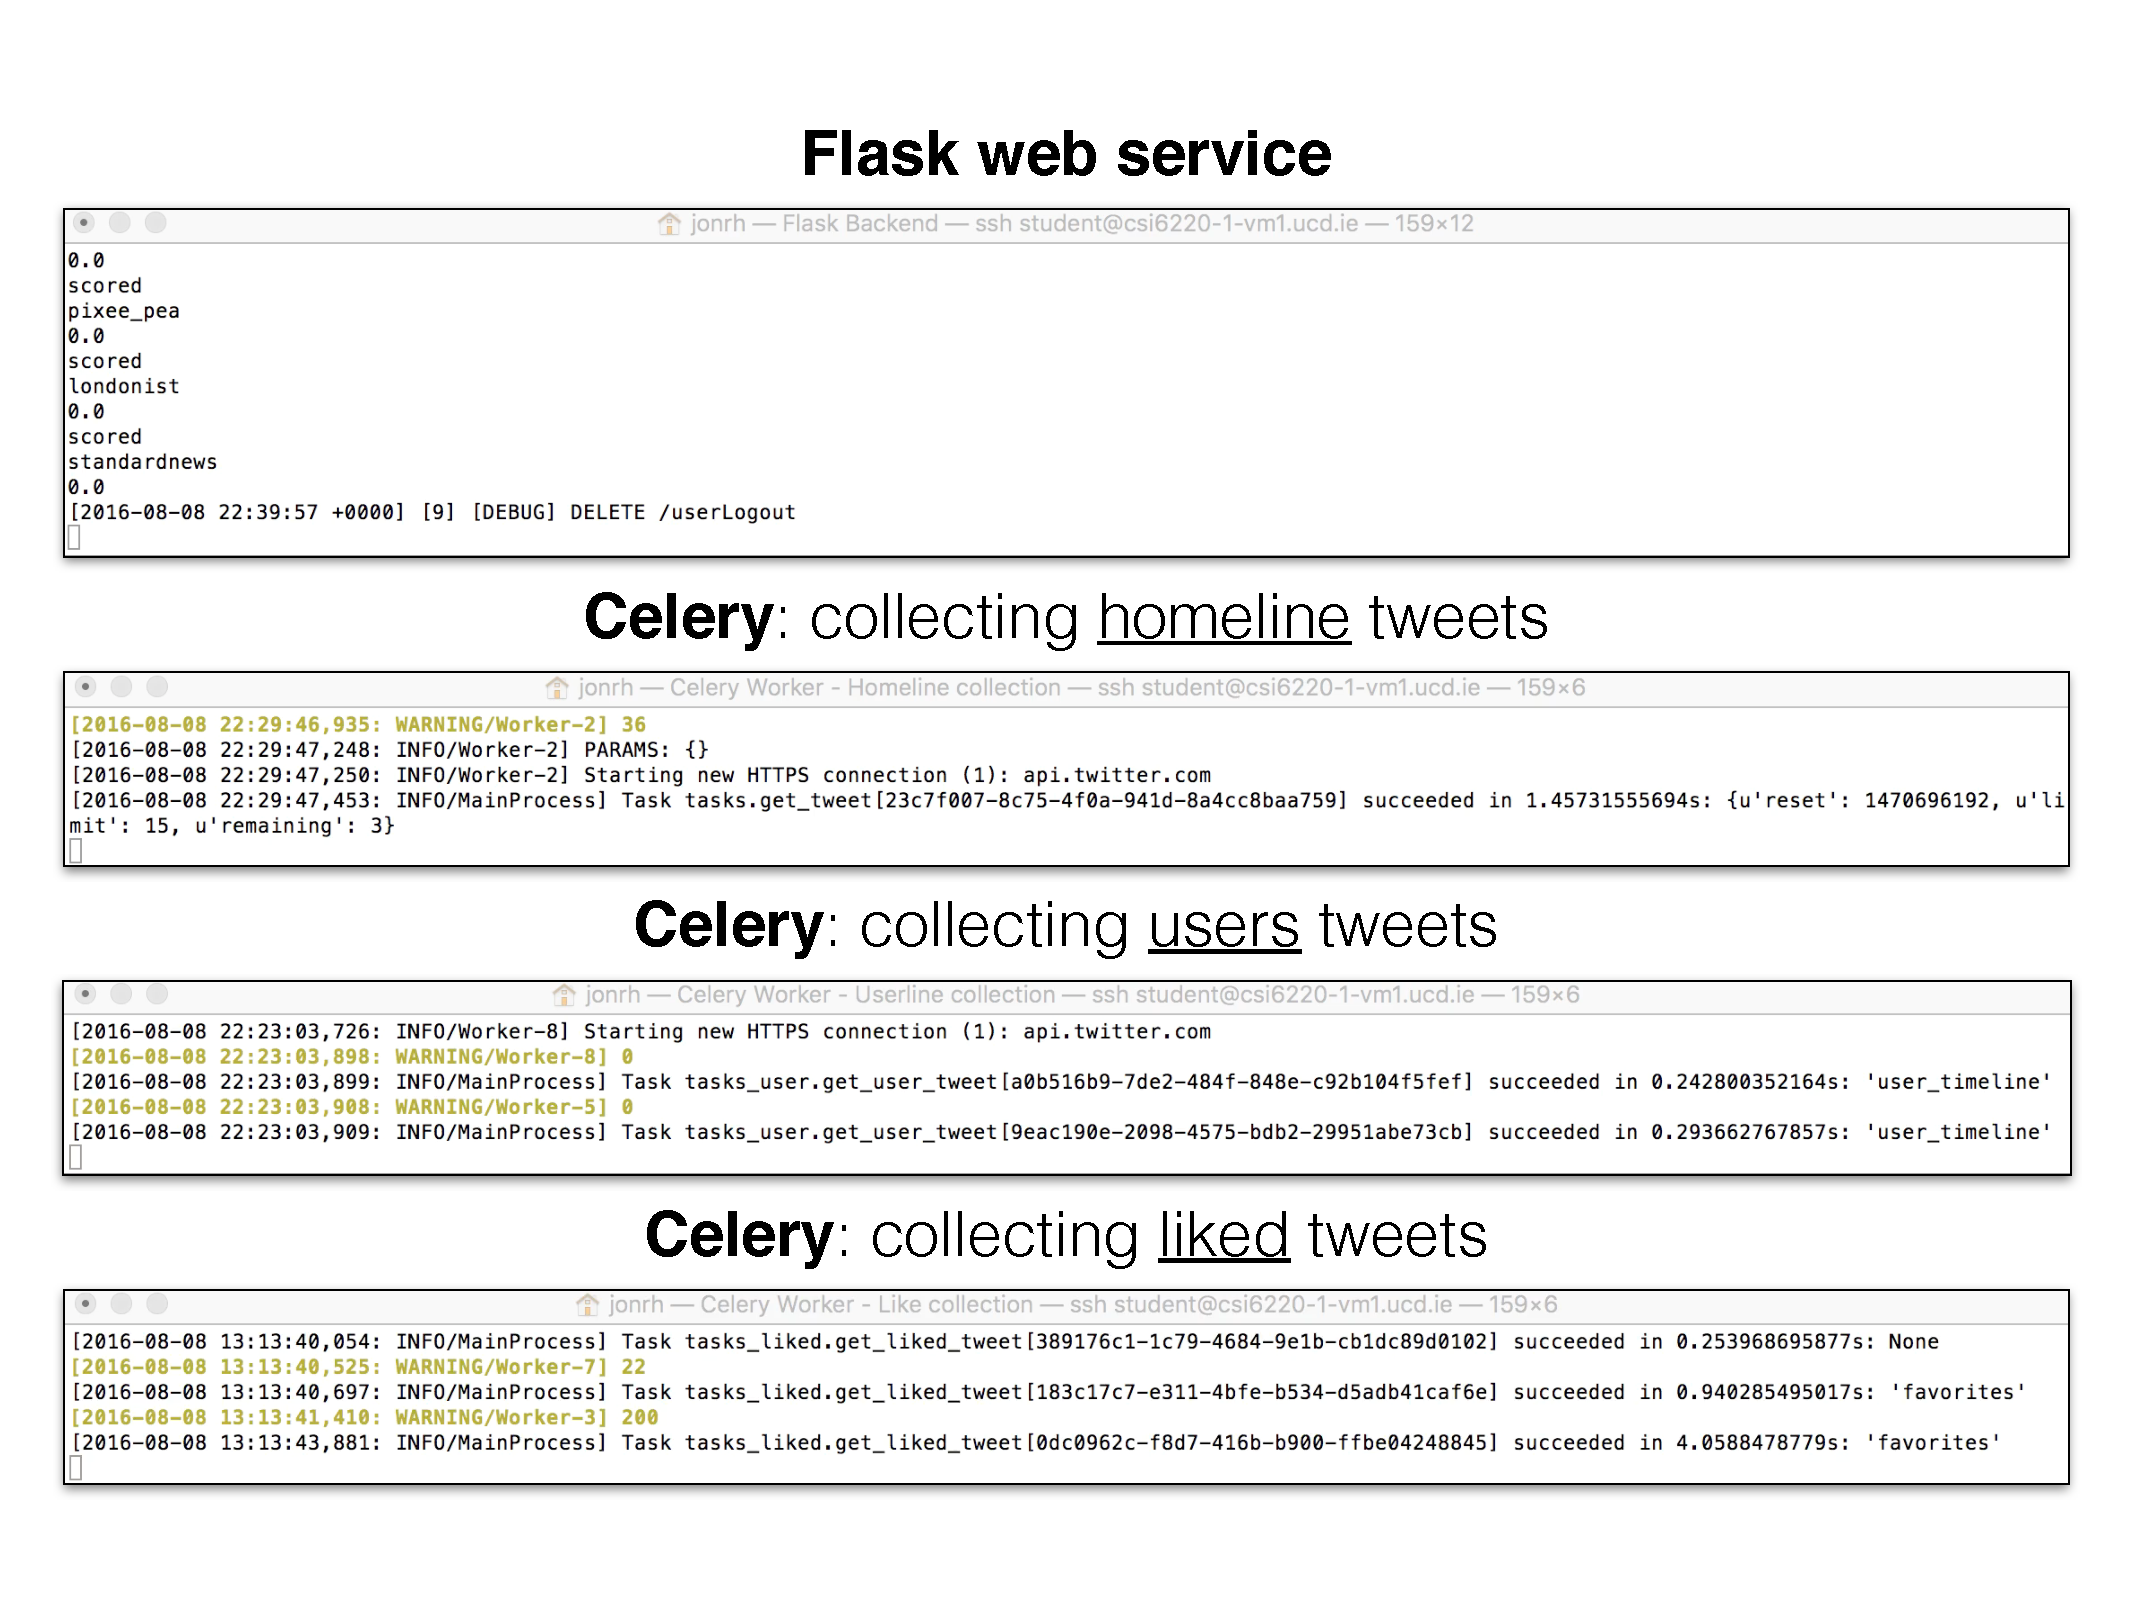
\includegraphics[width=\textwidth,trim={0 1cm 0 1cm},clip]{4containers}
    \caption{Screenshot of the four containers running in production}
\end{figure}

\noindent This was possible by overwriting the execution command when a container was started, a neat little re-use trick. An additional Redis container was used as a task queue for Celery (see \ref{celery}).

\subsubsection*{Development Workflow} 
Originally the backend was hosted on Heroku \cite{heroku} but due to monorepository requirements \cite{ll-blog-week9} we switched to our own continuous deployment (CD) workflow. After unsuccessful attempts\footnote{The SaaS providers used Docker v1.9.1 with a known race condition bug resulting in unstoppable containers for us. Jenkins and Docker v1.12 worked. See \cite{ll-blog-week9}\cite{ll-blog-week10}\cite{ll-blog-week11}.} with CircleCI \cite{circleci}, Distelli \cite{distelli}, and DockerCloud \cite{dockercloud} we settled on Jenkins \cite{jenkins}:

\begin{figure}[H]
    \centering
    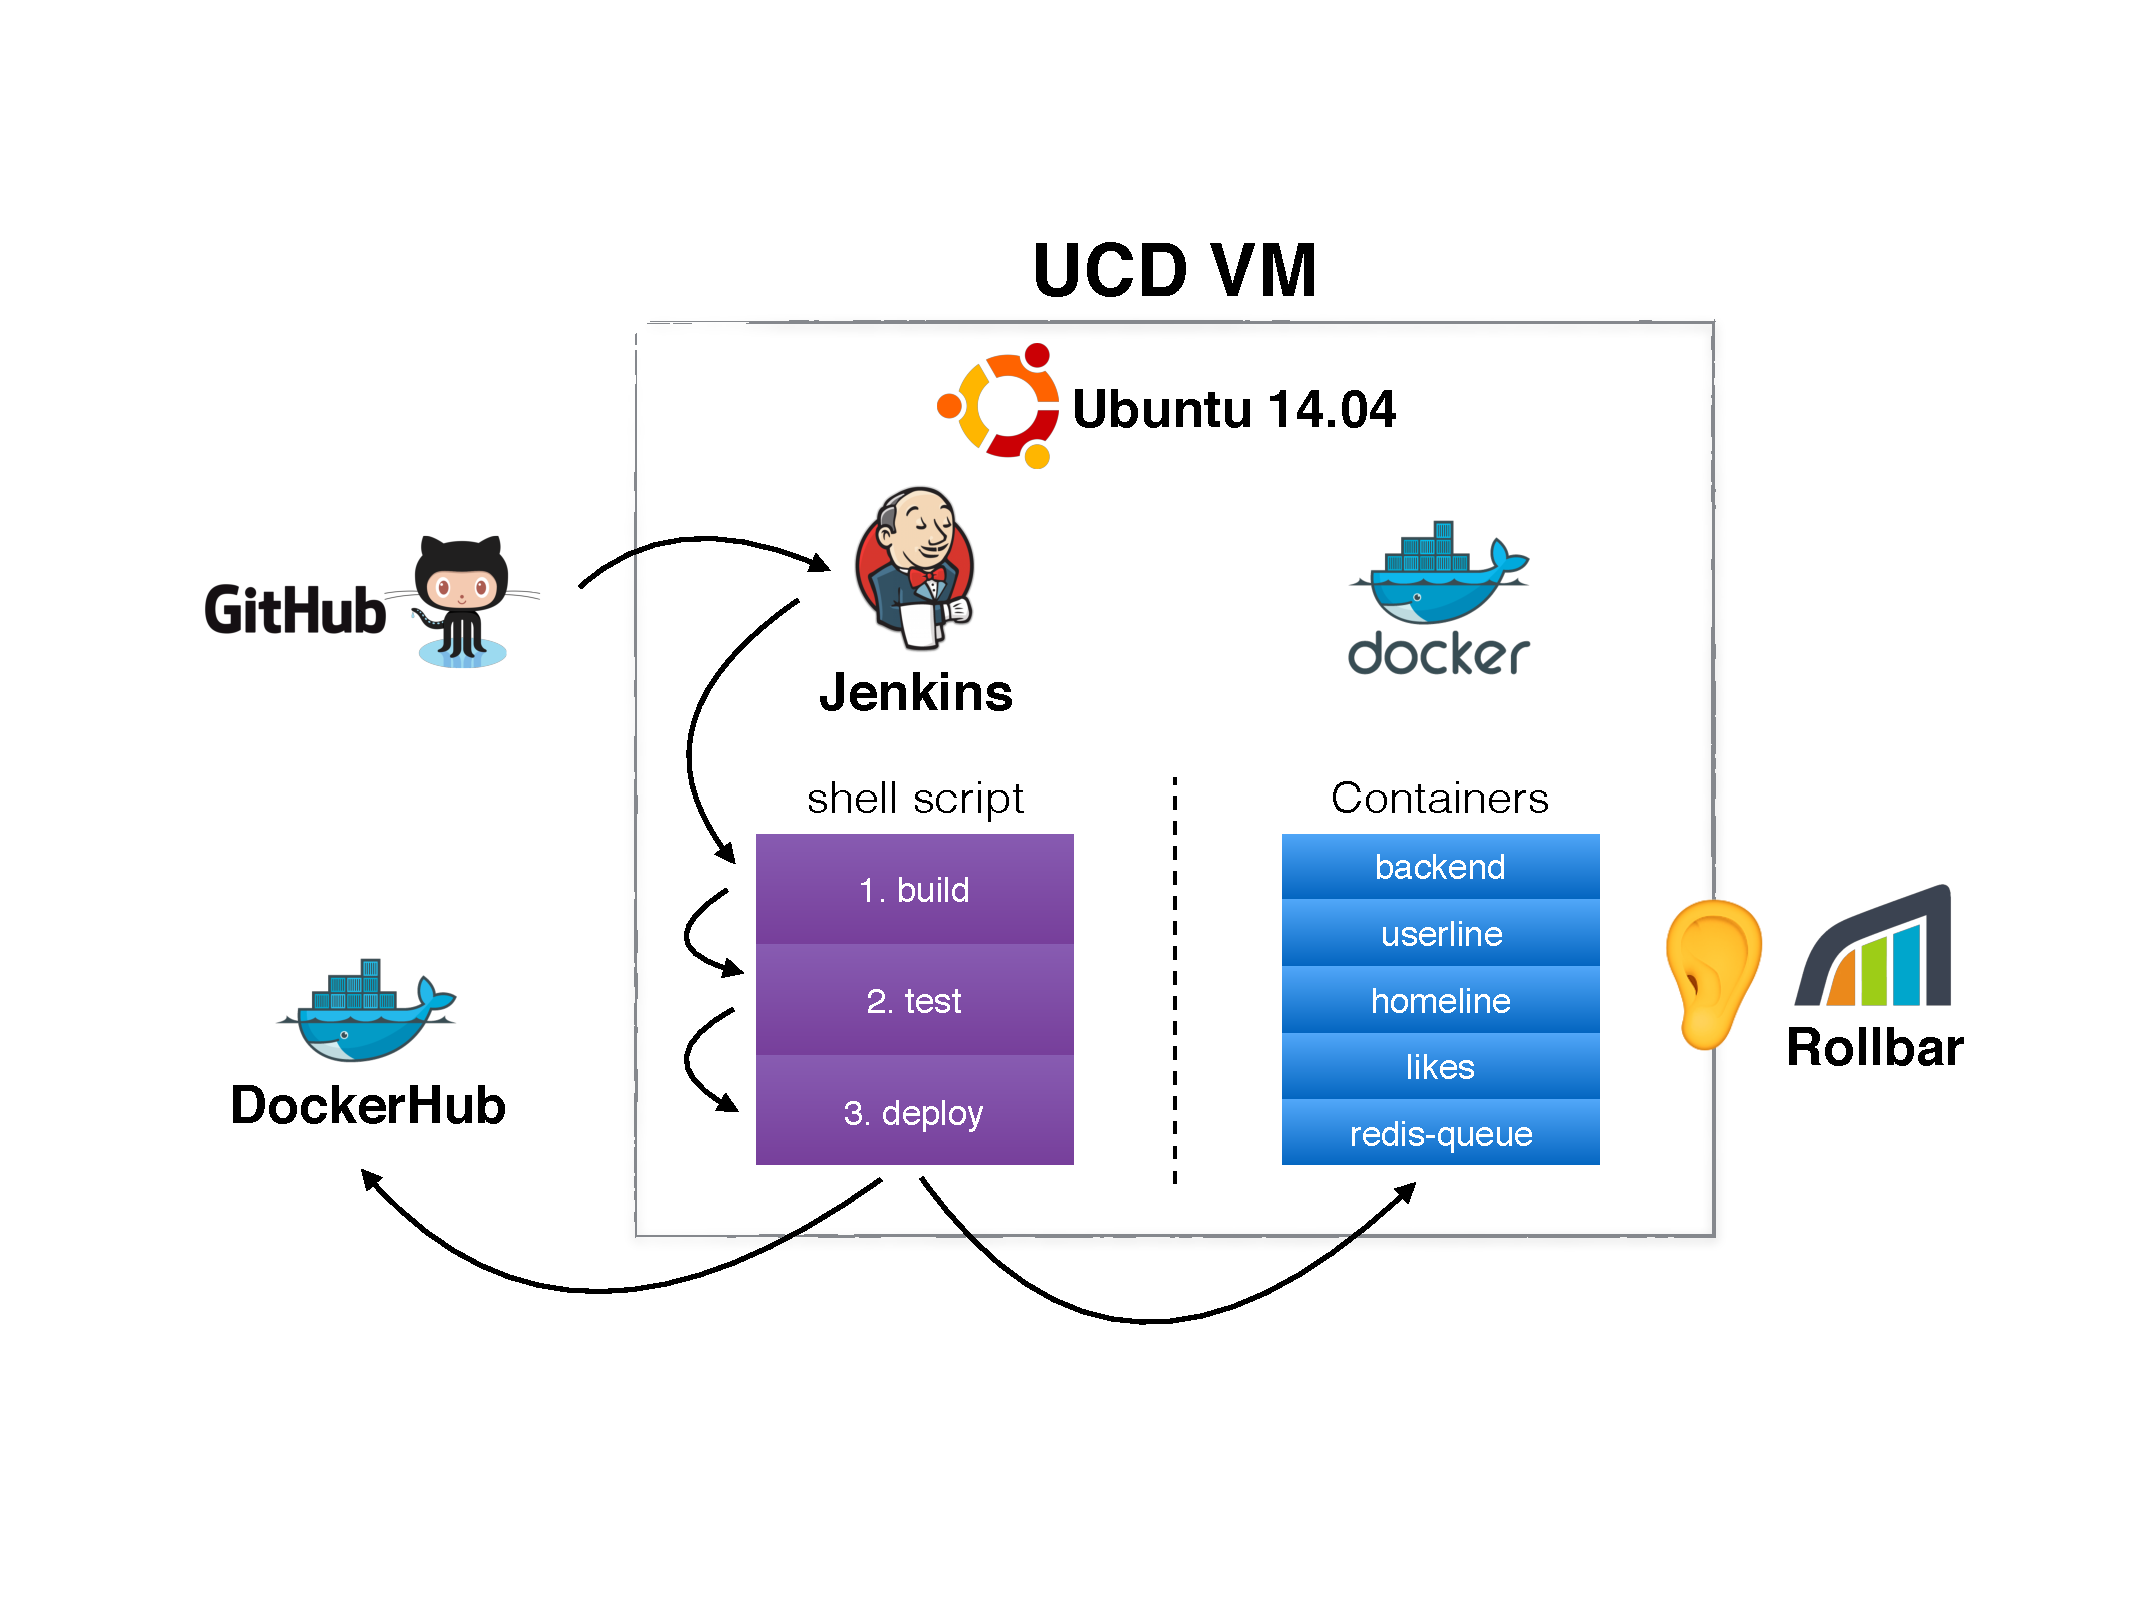
\includegraphics[width=\textwidth,trim={0 4cm 0 3.5cm},clip]{development_workflow}
    \caption{Automatic CD cycle on every Git push to the \textit{master} branch}
\end{figure}

\noindent Docker containers were built on every change and if tests passed the new version was automatically deployed and pushed to DockerHub. Just over 100 stable Docker images (deployable artifacts) were created during the project.

\subsubsection*{Web Server} 
For this project, three web frameworks were evaluated for the server: Django \cite{django}, Flask, and Bottle \cite{bottle}. Flask was chosen because it is more lightweight than Django and more popular and better supported (online resources, support, etc) than Bottle. Tweepy is used to interact with Twitter's APIs \cite{tweepy}.

The Flask Server is used to connect the iOS app, recommender system and the database with Twitters API. It handles requests from the iOS client and fetches the users personal timeline (Tweets posted by the user), their home timeline (Tweets posted by the user and the accounts they follow), their favourites (Tweets the user liked) and their profile from the Twitter API. This data is then stored in our RethinkDB database, and ultimately used in the recommender system to create tweet recommendations. The server also receives iOS client feedback from the user, stores it in the database, and retrieves it for use in the recommender system. The workflow of Flask is shown as below:

\begin{figure}[H]
    \centering
    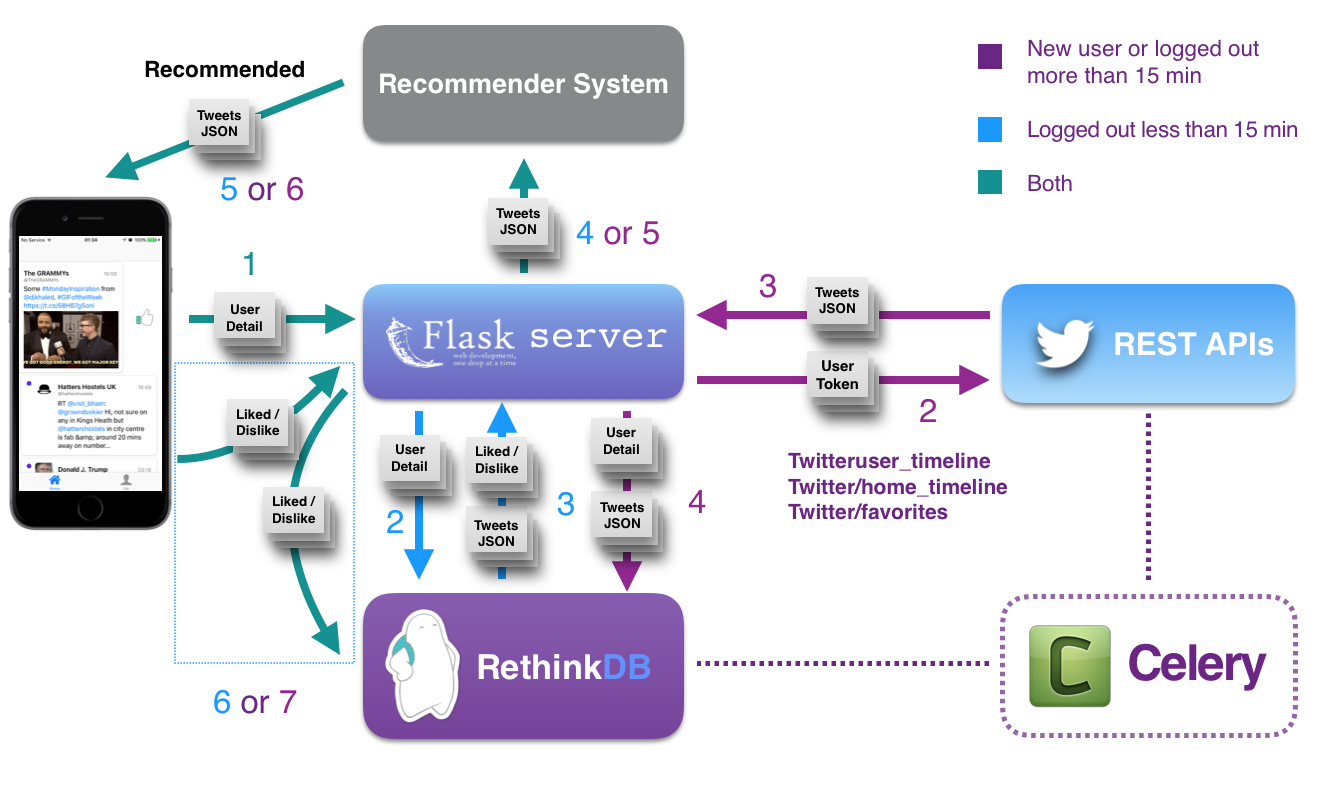
\includegraphics[width=1.0\textwidth]{flask_workflow}  
    \caption{Workflow of Flask server}
\end{figure}

As we can see, there are two situations when a user logs in. First, if the user is a new user or the user has logged out for more than 15 minutes, there will be either no record and tweets data of the user in the database or the tweets data is out of date, as Celery will stop fetching tweets if the user has logged out for 15 minutes. So the purple lines in the figure above will be executed. Flask will directly talk to the Twitter API acquiring for user’s home timeline, user timeline and liked tweets. After getting the data, the user’s token along with tweets data will be saved into database. Also, the running Celery works will start fetching tweets data for this user. The tweets data acquired from Twitter API in Flask will then be delivered to the recommender system for processing. Recommended tweets will be returned to the iOS client by Flask and the like/dislike data will also be recorded. 

However, if the user has logged out but it is still within 15 minutes, the blue lines in the figure will be executed. Flask will use the user detail to query the data in the database instead of Twitter API. This will avoid causing the rate limit error by sending too many requests to Twitter API.



\subsection{Data Sources, Collection \& Storage} 
There are two main data sources: the Twitter REST API and user feedback collected from the iOS client. We use the convenient third party library Tweepy to access the Twitter API. For example, the \textit{Cursor} \cite{cursor} object in Tweepy can implement the pagination of tweets in a single line of code, rather than manually using an iteration loop.

\subsubsection*{Rate Limits} 
To solve the rate limit challenge, we tried to find a way, which would continuously fetch data from the Twitter API without hitting the limits and persist it to a database. We came up with two potential solutions:

\begin{itemize*}
    \item Twitter Streaming API
    \item Twitter REST API + Celery
\end{itemize*}

\subsubsection*{Twitter Streaming API} 
The Streaming API gives developers low latency access to a stream of tweets. It provides three streams: 

\begin{itemize*}
    \item \textbf{Public Stream}: sample of public tweet streams
    \item \textbf{User Stream}: single-user stream
    \item \textbf{Site Stream}: like \textit{user stream}, but for multiple users
\end{itemize*}

\noindent For this project, \textit{site stream} would have been the most suitable option. Unfortunately at the time it was only available in a closed beta, which meant our only streaming option was the \textit{user stream}.

The \textit{user stream} contains roughly all of the data corresponding with a single user’s view of Twitter. We could then set up a stream for each of our users and collect our required data 24/7. Although the \textit{user stream} sounds like a very good choice, we found that the Streaming API also has rate limit. According to Twitter \cite{streaming}:

\begin{quote}
    \emph{\small Each Twitter account is limited to only a few simultaneous User Streams connections per OAuth application, regardless of IP. Once the per-application limit is exceeded, the oldest connection will be terminated.}  
\end{quote} 

Twitter didn’t specify the maximum number of connections allowed. However on the on Twitter's Developer Forum we learned that in practice each application is limited to about 10 - 20 simultaneous \textit{user streams} \cite{max}. If our application was ever to grow beyond a few users the \textit{user streams} would be completely inappropriate.
\\\\
We didn't want to introduce a new rate limit while trying to solve the first one. So we came up with the second solution -- Celery.	

\subsubsection*{Celery -- Distributed Task Queue} \label{celery} 
Celery is an asynchronous task queue based on distributed message passing. It is focused on real-time operation, but supports scheduling as well. We used Celery to set up a background task without affecting other requests of our app. As it supports scheduling, we can set up multiple periodic tasks, which keeps fetching data 24/7. The basic scenario is described in the figure below:


\begin{figure}[H]
    \centering
    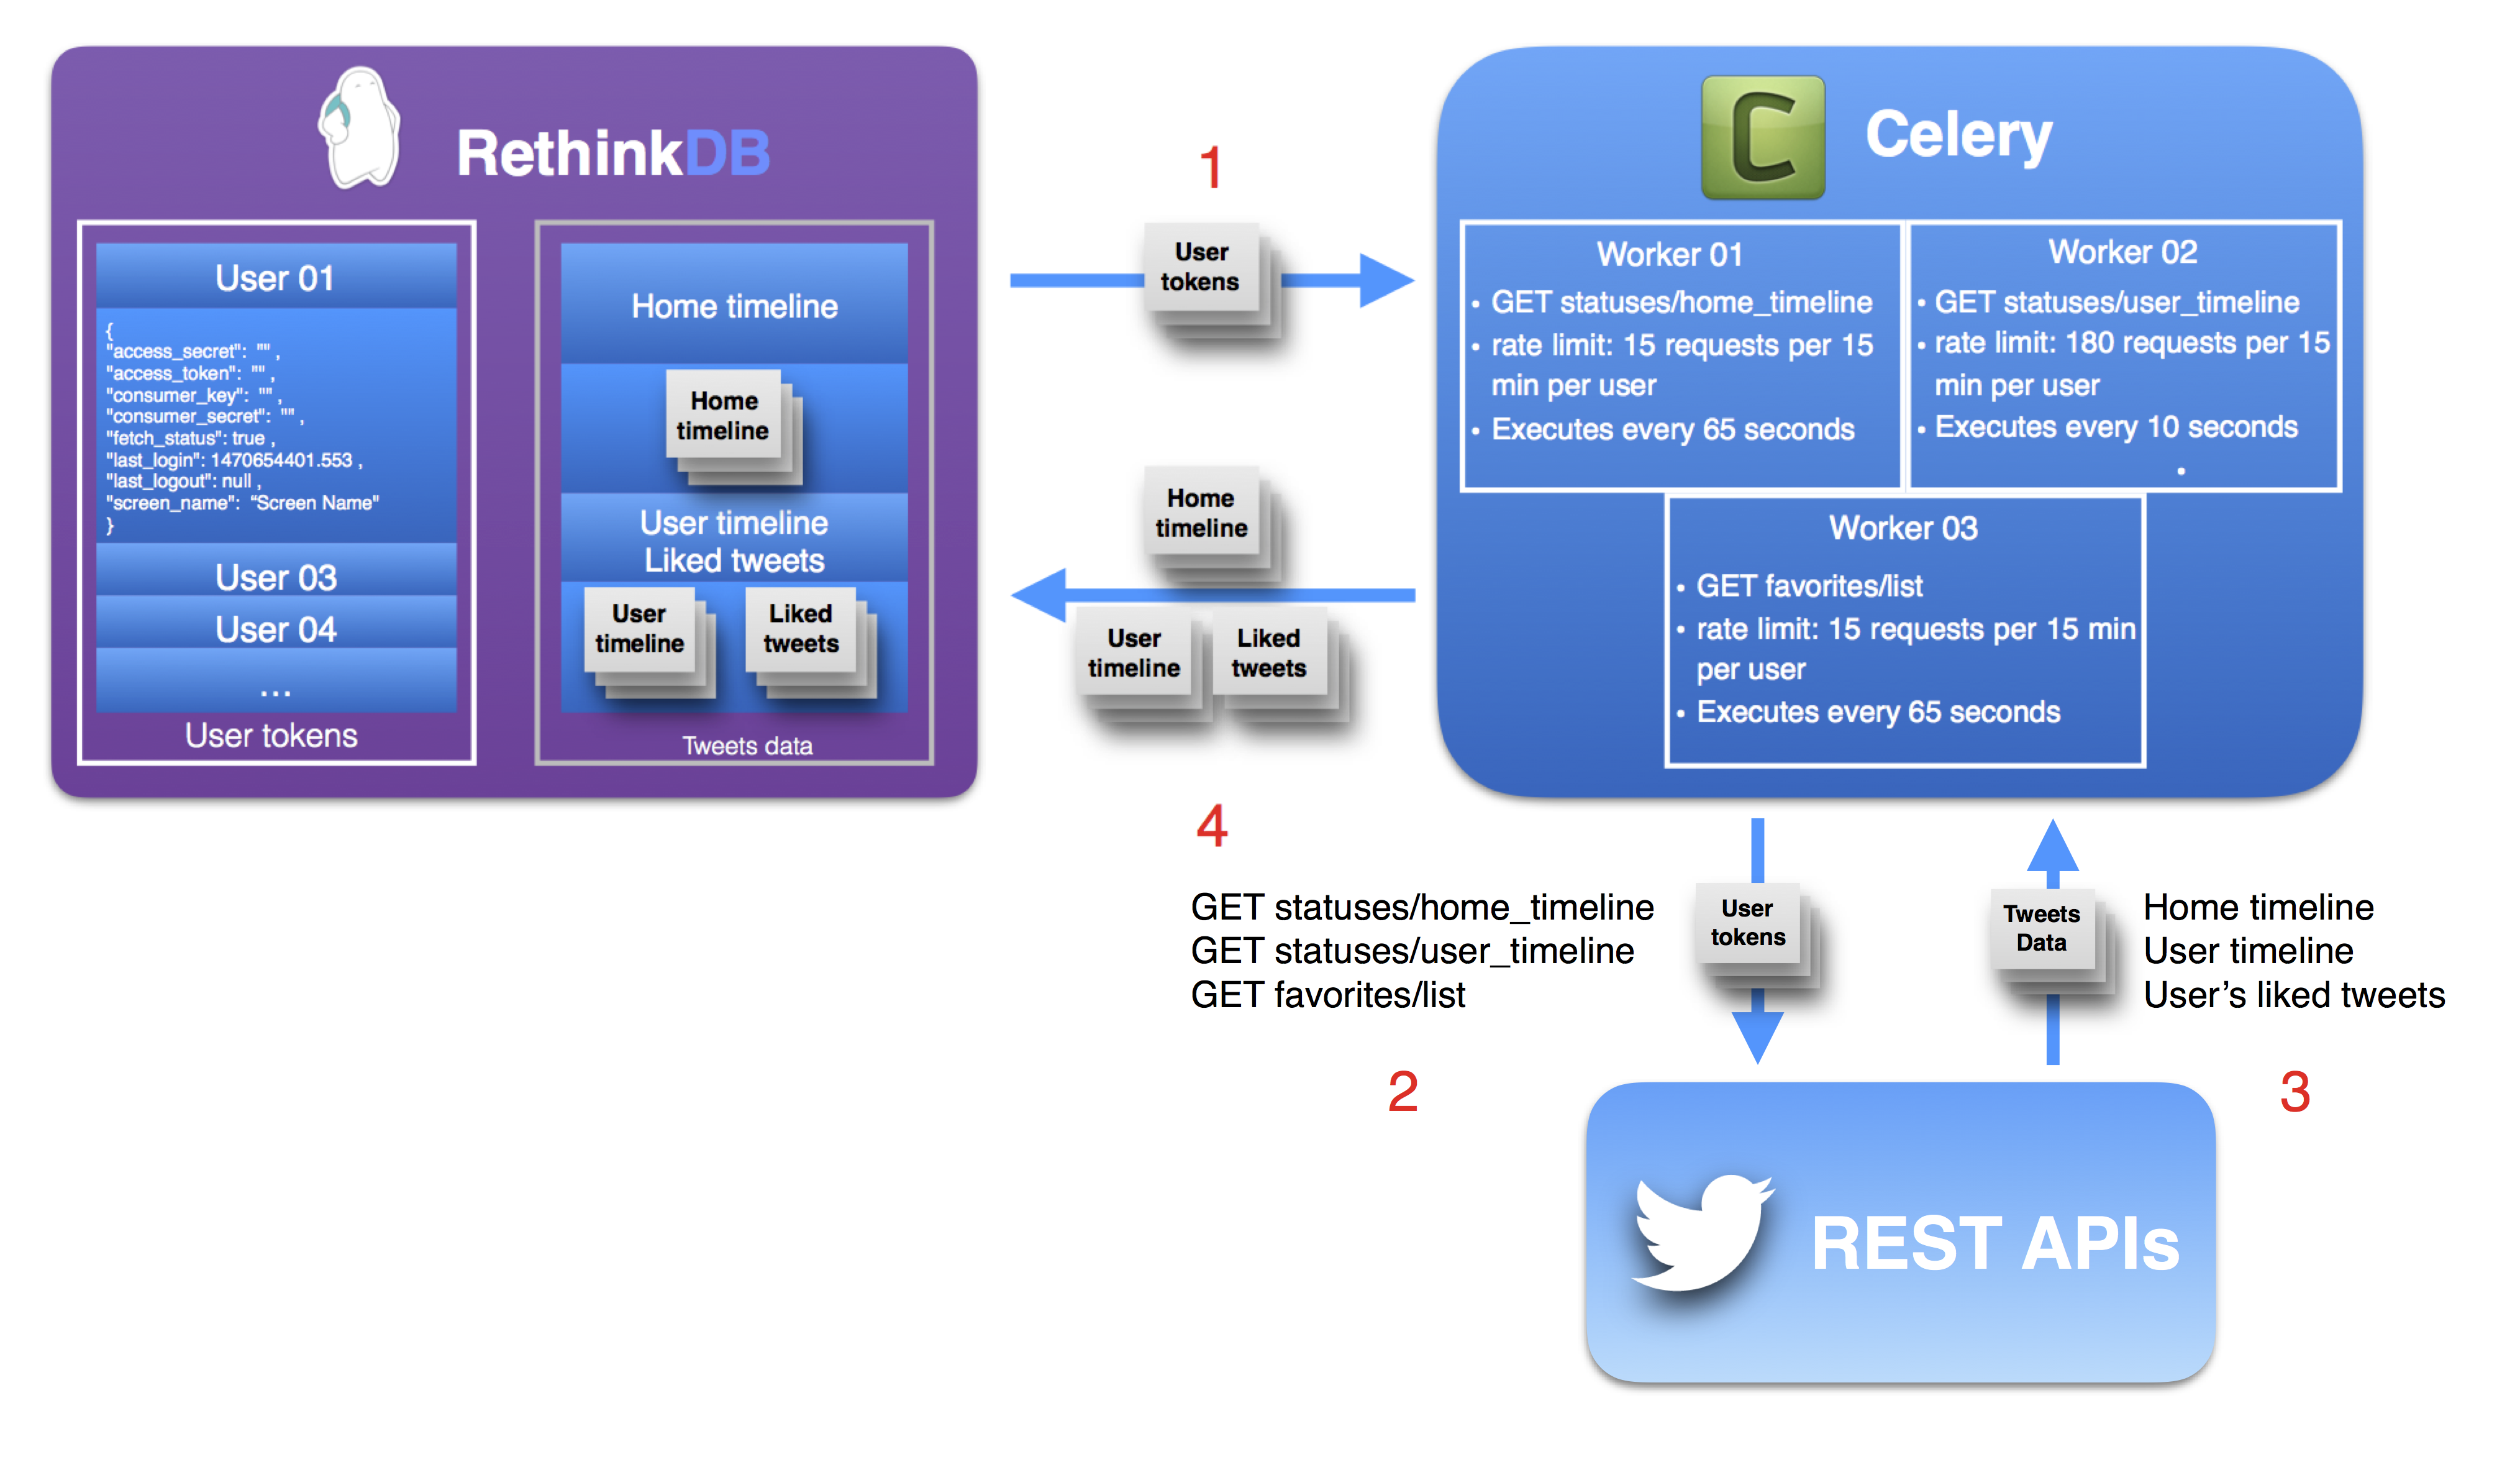
\includegraphics[width=\textwidth]{celery_scenario} 
    \caption{Celery workers in action}
\end{figure}

\begin{samepage}
\noindent There are three workers in Celery:

\begin{itemize*}
    \item \textbf{homeline}: collects tweets for display to a user
    \item \textbf{userline}: collects tweets \& retweets a user had created
    \item \textbf{favorites}: collects tweets a user has liked
\end{itemize*}
\end{samepage}

\noindent Each executes a task every 65 or 10 seconds to avoid hitting the rate limits. The tasks will first read all tokens from the table \texttt{"user\_tokens"} in the database. The table specifies whose tweets Celery should fetch and store. When a user logs in for the first time, the Flask server will insert the user’s OAuth token into the table. The format of each user tokens is stored as below:

\begin{samepage}
\begin{verbatim}
    {
        "access_secret":  "", 
        "access_token":  "", 
        "consumer_key":  "", 
        "consumer_secret":  "",
        "fetch_status": true,
        "last_login": 1470945465.371,
        "last_logout": 1470734005.455,
        "screen_name":  "lambda_lovelace"
    }
\end{verbatim}
\end{samepage}

\noindent Each task is executed asynchronously, so they won’t affect each other. When a user logs out, his \texttt{"fetch\_status"} in the table will be set to \textit{false} and the \texttt{"last\_logout"} time will also be updated. Therefore, Celery can check if the user logged out more than 15 minutes ago, if so, Celery will stop fetching data for the user, which can save a lot storage space. Tweet data collected is preprocessed then saved into the database. Each tweet collected will be saved as such:

\begin{samepage}
\begin{verbatim}
    {
        "screen_name":  "lambda_lovelace",
        "tweet": { ... },
        "tweet_id": 761591897626378200
    } 
    
    {
        "screen_name":  "lambda_lovelace",
        "tweet": { ... },
        "tweet_id": 761591275674079200
    }
\end{verbatim}
\end{samepage}

\noindent \texttt{"tweet\_id"}: primary key which is used to distinguish the tweets. \\
\texttt{"screen\_name"}: indicates whose timeline does this tweet belong to. \\
\texttt{"tweet"}: the tweet JSON object acquired from Twitter API
\\\\
With this Celery solution we have essentially manually constructed the \textit{site stream}. However there are some limitations. For example tweet delivery may be delayed by up to a minute. One workaround for that would be to have our iOS app make a direct User Stream connection to Twitter. However after a team discussion we decided not to do that because we believe that that the main purpose of our app is providing a better recommendation for the users, so one-minute latency is acceptable.

\subsubsection*{User Feedback Data} 
Whenever a user clicks the like/dislike button in the mobile app, the feedback will be sent to Flask and then be persisted into the database. Feedback is stored as JSON:

\begin{samepage}
\begin{verbatim}
{
    "currentUserScreenName":  "", //user using the app
    "feedback":  "dislike" ,
    "followerScreenName":  "LeapIN_EU", //user of this tweet
    "id":  "1fe778af-abd6-427f-bb77-962cb6449652", // RethinkDB ID
    "reason":  "Author", //reason of the user likes/dislikes
    "tweetContent": "", //actual text of the tweet
    "user_name":  ""
}
\end{verbatim}
\end{samepage}



\subsection{Recommender System} 
The recommender system is used to provide the personalised tweet home timeline for the iOS app. It performs filtering/personalisation on the users home timeline using a term frequency document created from the users personal timeline, feedback from the iOS client, and a variety of minor sources. Ultimately, tweets with higher overall ratings will appear first. This functionality is used by calling it's "generate" method. After filtering, the re-ordered timeline of tweets will be returned to the server and sent to the iOS client. The recommender system performs several minor functionalities in addition to it's main functions. For example, the age of a tweet is taken into account and slowly lowered as time passes, and the option to trim tweets that are X days old exists in the generate function. These minor functions are not covered in this section.






\subsubsection*{Twitter API} 
From the Twitter API, the recommender system uses both the users personal feed and their home timeline. That is to say, that the recommender system is fed this data through the Flask web server. It was decided to prevent the recommender system from making API calls about midway through the project development, as this would create inconsistencies in where data is stored and how it is accessed. The main use of the personal timeline is in the creation of the Term Frequency document and the "second net" Term Frequency document. The main use of the users home timeline is to provide a set of tweets to perform recommendations upon.

\subsubsection*{iOS client feedback} 
iOS client feedback consists of tweet data that allows users to indicate whether they like or dislike the content of the tweet or the tweets author. The effect that content feedback has on the users preferences essentially works by “balancing” the term frequency document. By this, we mean that if a tweet containing a term frequency document term is liked for it’s content, the weighting of that term will go up while the rest of the terms take a minor decrease (Combined, all decreases are proportionate to the increase). 
\\\\
Author sentiment is totalled up by the number of likes or dislikes they were given, and the overall sentiment is used when weighing a tweet. For example, if the overall sentiment is bad for an author, the tweet weight will be negatively affected. If it is mixed, then tweet weight will be either positively or negatively affected, but in a minor manner.

\subsubsection*{Term Frequency Document} 
The term frequency document is derived from the users personal timeline. Using a Counter object, a cut-off point for the number of terms and an exhaustive list of English stop-words, the term frequency document creates a list of the most occurring words that appear in a users personal timeline, excluding stop-words. A cut-off point is used (Roughly twenty is ideal, based on trial and error) to prevent the term frequency document from holding all the non-stop-word terms in the user personal timeline. For example, if the cut-off point was three and the term frequency document preliminary list contained five terms, the cut-off point would ensure that the term frequency document only held the top three terms from the preliminary list. A numeric scale value (10.0) provides the total “chunk” that each term takes up. This means that each term takes up a value out of a total (10.0). This approach allowed us to value terms relative to each other.

\begin{figure}[H]
\centering
\begin{verbatim}
                    {
                        u'ruby': 0.10, 
                        u'hacker': 0.30, 
                        u'software': 0.50, 
                        u'programming': 0.20, 
                        u'twitter': 0.81, 
                        u'springframework': 0.40, 
                        u'api': 0.10, 
                        u'code': 0.20, 
                        u'python': 0.40, 
                        u'java': 4.28
                    }
\end{verbatim}
\caption{An example term frequency document.}
\end{figure}


\subsubsection*{Second Net} 

The recommender systems Second Net feature largely performs the same functionality as the term frequency document. It is essentially a term frequency document that has a cut-off point twice the size of the original term frequency document. The purpose of this "secondary" term frequency document is to attempt recommendations on tweets that did not contain any of the original term frequency documents terms. This works by separating the recommendation list into two sets, those that contain terms from the original term frequency document, and those that do not. Sorting is performed on the former using the original term frequency document, and on the latter using the second net term frequency document. The results of the second net sorted list are appended onto the end of the list containing terms from the original term frequency document. This gives us a list containing firstly the higher quality recommendations using the original term frequency document, followed by progressively lower quality tweets that use the second net term frequency document.

\begin{figure}[H]
\centering
\begin{verbatim}
                    {
                        u'ruby': 0.10, 
                        u'pwned': 0.05, 
                        u'testing': 0.15, 
                        u'hacker': 0.30, 
                        u'software': 0.50, 
                        u'programming': 0.20, 
                        u'twitter': 0.81, 
                        u'springframework': 0.40, 
                        u'api': 0.10, 
                        u'code': 0.20, 
                        u'android': 0.20, 
                        u'ruby': 0.20, 
                        u'python': 0.40, 
                        u'java': 4.28, 
                        u'website': 0.35, 
                        u'wordpress': 0.15, 
                        u'tweet': 0.70, 
                        u'automated': 0.10, 
                        u'soccer': 0.05, 
                        u'geeks': 0.05
                    }
\end{verbatim}
\caption{An example of what the previous term frequency document's second net could look like.}
\end{figure}
    



\newpage
















































\section{Evaluation} 

\subsection{Hypothesis}








For the experiment the main question is: 

\begin{center}
    ``\textit{Is $\lambda$ Lovelace's personalised tweet feed \\
    more interesting or relevant to the user than the \\
    default chronologically ordered tweet feed from Twitter?}''
\end{center}

Our goal was to show that it can be preferable for the user to have short-term recommendations. In essence, we want to provide users with a personalised timeline that, when compared to the Twitter home timeline, will be chosen over twitters offering. We believe that the hypothesis is an important question to ask, due to both the ubiquitous nature of Twitter and the powerful effect of recommender systems. Entire businesses revolve around the strength of their recommender systems, so we want to attempt to marry the popular platform of Twitter with the personalisation of recommendation.

\subsubsection*{Related Work} 
In the course of the creation of this experiment, we identified three particularly interesting examples of similar experiments, relevant to the experiment that we performed. In \textit{Towards a Followee Recommender System for Information Seeking Users in Twitter} \cite{paper1} the authors perform a very similar experiment to ours, with the exception of the data collection section, and found success. The authors asked twenty-six users the following question: "Would you have followed this recommended user in the first place (when selecting which users to follow in the first part of the experiment), if you had know this account?", while tracking their answers. While both us and the authors take a quantitative approach to our experiments, Marcelo G. Armentano et. al required users to perform these tests on a desktop computer. This approach is much easier to implement than our use of multiple mobile devices. 

This paper also describes how the authors requested that users create new accounts with fresh data. This approach, although not applicable to our system, would have been more convenient for testing purposes if our system did not require power users. "Power users" being regular Twitter users that generally follow hundreds of accounts and have hundreds of tweets, retweets and likes. This type of user account us completely different from the accounts used in the previously mentioned experiment. Overall this is a very similar testing approach to ours, as the system tested also provided somewhat similar functionality, that of twitter recommendations.
\\\\
This paper provided us with a rough idea of how we should proceed with this experiment and generated several ideas for the experiment. Most of which were ultimately not used.
\\\\
In \textit{Recommending Twitter Users to Follow Using Content and
Collaborative Filtering Approaches} \cite{paper2}, the authors perform two forms of testing, a preliminary offline experiment and a live user trial experiment. This allowed the authors to make initial assumptions on their project before beginning the live user trials, which would be more difficult to organise and take more effort. It was a much "safer" choice to hold a preliminary experiment before the main experiment. Similarly to the previous paper, the authors of this paper simply had users perform actions (based on questions) with their system and record the results. This paper highlighted the need for us to hold preliminary trials for our experiment, so that the main experiment would not be "wasted".
\\\\
In \textit{Using Twitter to Recommend Real-Time Topical News} \cite{paper3}, the authors tackle a similar topic to \textit{Towards a Followee Recommender System for Information Seeking Users in Twitter}, but perform user testing over a period of five days. This setup allowed the authors to gain data outside of a testing environment. Authors basically requested that users used their system as their default RSS reader while they went about their day-to-day activities, and based their metrics on user click-throughs. This means that the authors based success on how much more users used their system than their original RSS reader.Although this environment would be much more difficult to enforce upon participants, it gave the authors more data in a more natural environment for the user. 

We incorporated an aspect of this open style of testing by allowing participants to come and test over a period of several hours, rather than a scheduled approach. This paper also highlighted a discrepancy between what the participants say they prefer, and what they actually prefer when dealing with content recommended from twitter or content that is followed by their twitter friends. This influenced us to use more objective methods when testing.




\subsection{Experimental Method}
\subsubsection*{Overview} 







For this experiment, we prepared an evaluation-specific version of our mobile app. The app allowed participants to rate individual tweets if they were interesting or relevant to them: thumbs up, neutral or thumbs down.

\begin{figure}[H]
    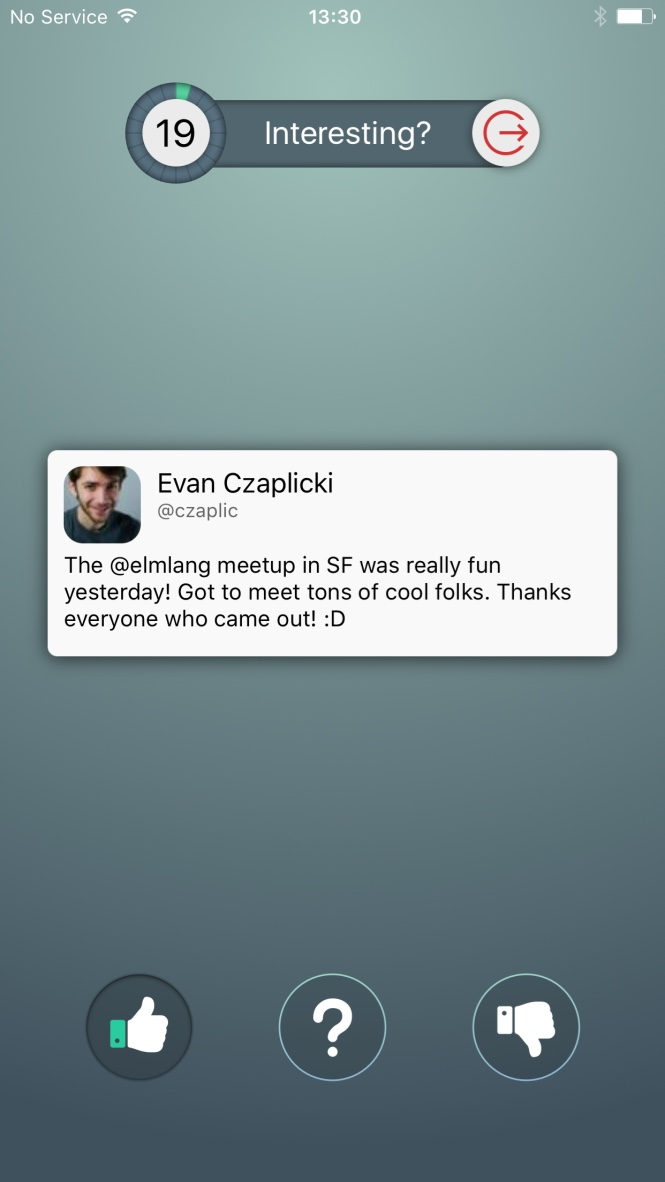
\includegraphics[width=0.4\textwidth, center]{eval1}
    \caption{Screenshot from the evaluation iOS app}
\end{figure}

Each evaluation run had the user rate two batches of 50 tweets at a time, that is each user rated 100 tweets in total. Each batch of 50 tweets was sourced from two feeds. The 25 newest tweets are taken from Twitter's chronologically ordered feed\footnote{in the Twitter API this is referred to as the \textit{homeline}} and the other 25 tweets are taken from $\lambda$ Lovelace's feed. The order was then randomised so the evaluator did not know from which feed the tweet came.


\begin{figure}[H]
    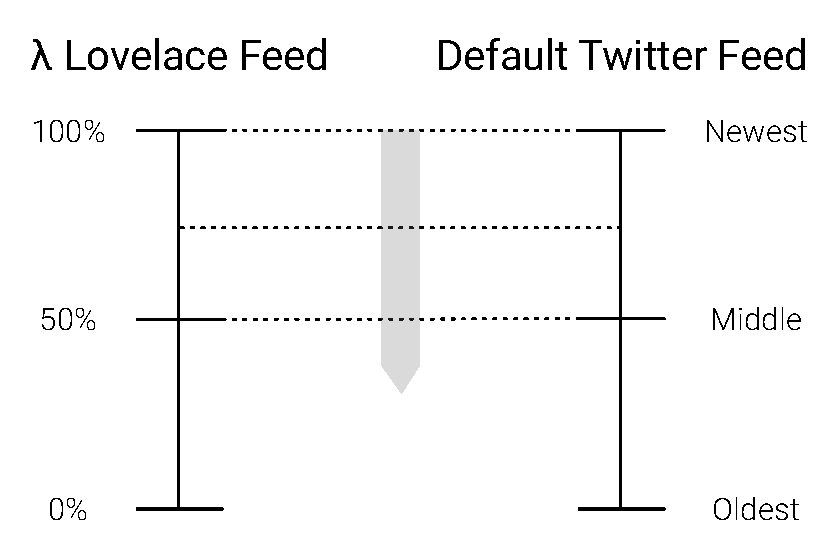
\includegraphics[width=0.6\textwidth, center]{evaluations_1}
\end{figure}

From the data gained from this experiment, we hoped to draw conclusions on the quality of our recommended tweets. For these purposes, participants had to log into the the evaluation app with their personal Twitter account.
\\\\
Participating subjects were largely drawn from college-aged students who are familiar with Twitter, allowing us closer access to the power users that this system is aimed at. This experiment took place in B0.02 of the Computer Science and Informatics building on University College Dublins Belfield campus, allowing for a short travelling distance, ample room for potentially large numbers of participants and an organised environment. The expriment took place on August 5th, from 11AM to 4PM, although it is worth noting that the actual participants appeared only on August 8th.
\\\\
Metrics used for this experiment were drawn from the results of the evaluation app. These metrics reflect sentiment for batches of tweets from both the original timeline and our recommender system. Tweets either have positive(liked), negative(disliked) or neutral(neither) sentiment. The score of both the recommender system and the original timeline is tallied up to discern the more well-received system.

\subsubsection*{Data Collection} 









Data collected by the participants is of a quantitative nature, where we can view the results of each evaluation and infer preference for either the official Twitter timeline, or our feed. The metrics used are numerical, with each like adding to the "score" of either the official Twitter timeline or our evaluation app. We intended to capture the users interests with the recommendations provided, so should be scored higher than the default Twitter timeline.
\\\\

From this data, we were able to compare our recommendations with Twitter's chronological tweet feed. Finally, from this comparison it was somewhat determined which form of Twitter feed provides more value to the user. 

\\\\


The collected data was stored in RethinkDB\footnote{a document database where each "row" is a JSON object} so that it was accessible in the same manner as both the live and test tweet data sets.


\begin{samepage}
\noindent Here is a pseudo example JSON data submitted for an evaluation run:
\begin{verbatim}
{
    "id": "4c1c9819-df34-4803-9678-fbeab7641c02",
    "time": 1469724613038,
    
    "user_info": {
        "screen_name":  "lambda_lovelace",
        "tweets_liked": 1337,
        "tweets_of_me": 824,
        "users_following": 432
    },

    // Aggregate tally of results for this evaluation run
    "counts": {
        "originalDislike": 3,
        "originalLike": 4,
        "originalNeither": 3,
        "recommendDislike": 2,
        "recommendNeither": 4,
        "recommendLike": 4
    },
    
    "result": [
        {
            "source": "original", // Twitters default feed
            "tweetId": "758705114785910785",
            "userOption": "like", // User liked the tweet
            "userScreenName": "@smarimc"
        },
        
        ... // 19 other tweets
    ]
}
\end{verbatim}
\end{samepage}

\subsubsection*{Selected Subjects} 





Subjects for the pilot evaluations were chosen from amongst team $\lambda$ Lovelace's family, friends and acquaintances. This was not a part of the main experiment for this project, due to the bias present in this group and the relative lack of good-quality participants.
\\\\
This preliminary experiment served as a filter for the main experiment. In this first experiment it was hoped that outsider perspectives would reveal issues with the software that we did not initially notice. As there was a limited amount of time left for this project, we were constrained in how many of the main experiments we could hold, so the preliminary was vital to preventing fundamental error in the main experiment. 


\\\\
Participants were obtained through fliers distributed throughout the University grounds that advertised the experiment for August \nth{5}. 




\begin{figure}[H]
    \centering
    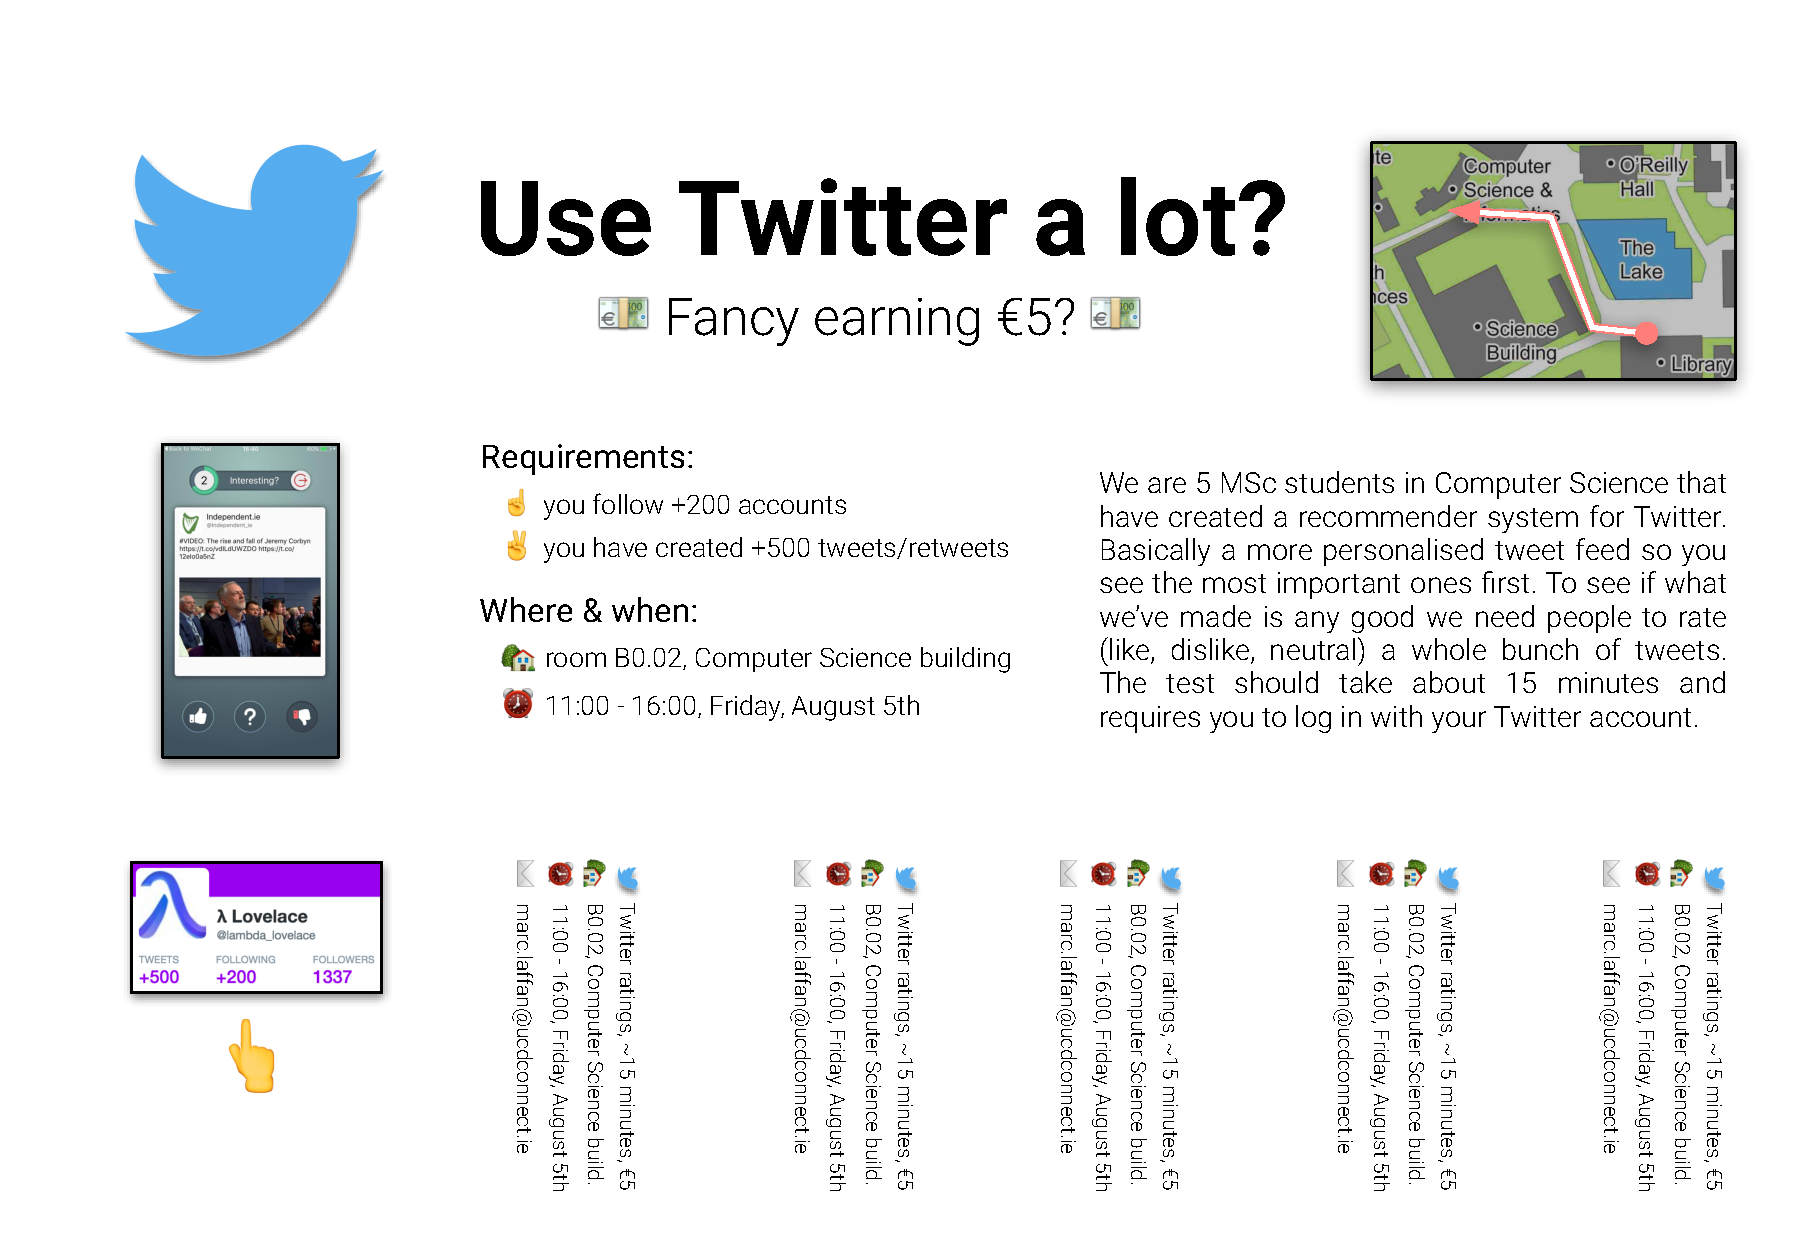
\includegraphics[width=0.8\textwidth]{evaluation_poster}
    \caption{The evaluation flier we posted on noticeboards outside James Joyce library on the UCD campus. For a full size please see Appendix \ref{full-size-poster}.}
\end{figure}




\subsubsection*{Data Analysis} 





We brainstormed upon this several times and ultimately decided to take the simplest approach. That is, we compared our version of the Twitter feed to the default home timeline. The version that gained more "likes" and less "dislikes" in the evaluation app was judged the better version with concerns to relevancy. Thus answering this papers original question of "\textit{Is $\lambda$ Lovelace's personalised tweet feed more interesting than the default chronologically ordered tweet feed from Twitter?}" with hard data.
\\\\



Tasks were intentionally left simple, as requesting more complex tasks from participants can lead to pitfalls in experimentation, as seen in \textit{Using Twitter to Recommend Real-Time Topical News} \cite{paper3}, where participants voiced an opinion that later revealed to be entirely untrue.
\\\\
This form of analysis, due to its numerical data, also allowed us to graph the resulting dataset for comprehension purposes. 









\subsubsection*{Practical Setup} 







The experiment was run within room B0.02 in the Computer Science building at University College Dublin. The purpose of this setup was to allow participants ease of access for the duration of the experiment. Believing that fewer barriers for participation will yield higher turnout, we allowed participants to show up at their convenience to prevent the discouragement that presents itself in strict scheduling for an experiment. 




The choice of room was both a convenient choice and an appropriate one. The rooms in the ground floor of the Computer Science and Informatics building have been used before for University College Dublin's end-of-semester exams. 


\\\\
The app was ready to run on three of team $\lambda$ Lovelace's iPhone devices, so that there was no need for the participants to install the software. This was intended to speed up the experimentation process, and further remove barriers to entry for the user. The only thing the user was required to do was sign in with their own Twitter credentials and perform runs with the evaluation app.
\\\\
In addition to running the experiment in person, we published the evaluation app via the beta mobile app distribution platform HockeyApp \cite{hockeyapp}. The team got it running successfully but the pilot evaluation revealed the process was too cumbersome and time-consuming to be practical for the experiment.


\\\\
As a result of the pilot experiments amongst friends and family, we found that one-hundred tweets was the ideal number for the user to evaluate. From beginning to finish, the users took about fifteen minutes to complete the experiment. This consisted of our explanation of the app and what was expected of the participant, logging the user in and rating the tweets themselves. 



\subsection{Evaluation Conclusion} 







Unfortunately, on the day of the experiment we found that no-one was interested in attending. Fortunately, students were interested enough in the experiment that we could schedule two participants on the \nth{8} of August in the same setting. 


\\\\
We were able to answer the question in this sections hypothesis with a resounding "yes", but with a caveat. Almost all users (Friends and family included) found our recommended tweets preferable. However, we identified a type of user that uses twitter for a singular purpose/topic and found that they had an overwhelmingly positive preference for our recommendations instead.
\\\\



Given more time, an ideal experiment setting would involve allowing the participants to use our app over the course of several days. Our app could have temporarily replaced the participants use of the official Twitter website and the users could respond at the end of a week with their level of satisfaction with the app. Further testing could involve requesting participants to give their level of satisfaction on a daily basis, with us tweaking several of the attributes of the recommender system (Number of terms in the term frequency document, values given to hashtags and liked/disliked tweets, etc) and observing the effect on participants satisfaction levels. This form of testing is not without its disadvantages, as participants can give inaccurate feedback when critical thinking is involved. However this could be circumvented, resources permitting.
\\\\
Overall, this experiment was useful for the purposes of evaluating our application. However like most endeavours, there will always be space for improvement. 

\begin{figure}[H]
    \centering
    \includegraphics[page=6,width=\textwidth]{evaluation_charts}
    \caption{Total aggregate of likes/dislike/neutral for all evaluation runs}
\end{figure}


\begin{figure}
    \centering
    \begin{subfigure}[b]{0.48\textwidth}
        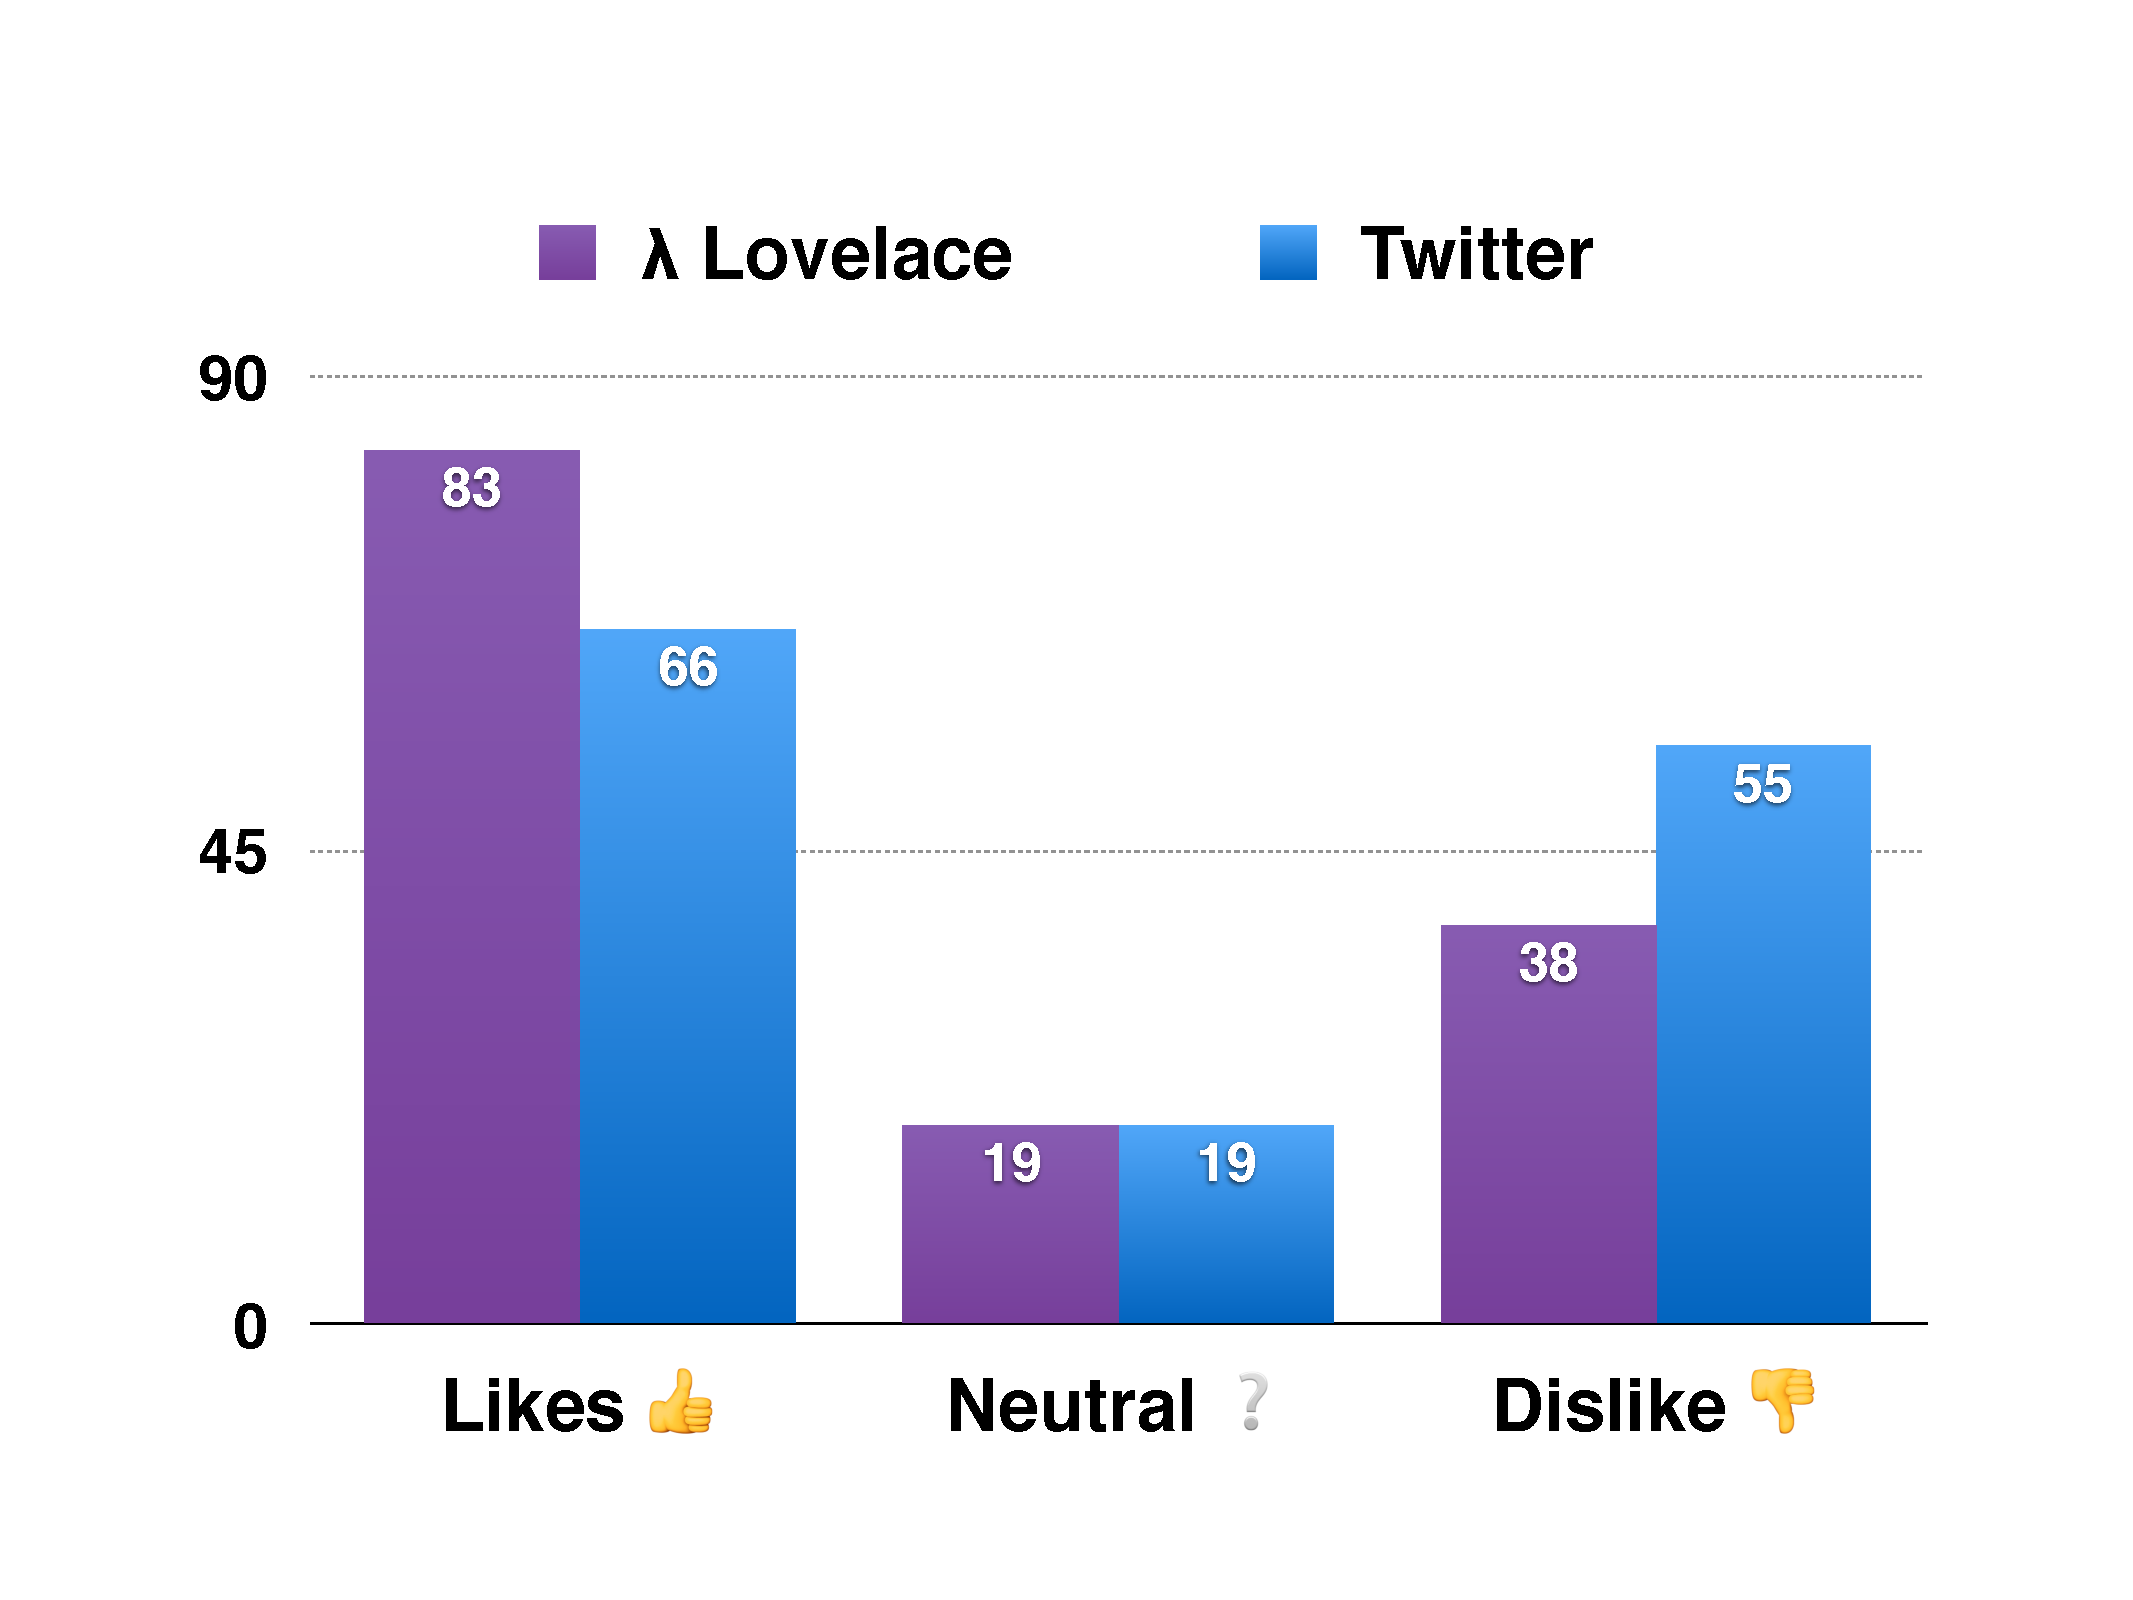
\includegraphics[page=1,width=\textwidth]{evaluation_charts}
        \caption{participant \#1}
        \label{fig:participant1}
    \end{subfigure}
    ~ 
      
    \begin{subfigure}[b]{0.48\textwidth}
        \includegraphics[page=2,width=\textwidth]{evaluation_charts}
        \caption{participant \#2}
        \label{fig:participant2}
    \end{subfigure}
    
    \vspace{2em}
    
    \begin{subfigure}[b]{0.48\textwidth}
        \includegraphics[page=3,width=\textwidth]{evaluation_charts}
        \caption{participant \#3}
        \label{fig:participant3}
    \end{subfigure}
    ~
    \begin{subfigure}[b]{0.48\textwidth}
        \includegraphics[page=4,width=\textwidth]{evaluation_charts}
        \caption{participant \#4}
        \label{fig:participant4}
    \end{subfigure}
    
    \vspace{2em}
    
    \begin{subfigure}[b]{0.48\textwidth}
        \includegraphics[page=5,width=\textwidth]{evaluation_charts}
        \caption{participant \#5}
        \label{fig:participant5}
    \end{subfigure}
    
    \vspace{2em}
    
    \caption{Individual results from participants}
    \label{fig:evaluation-results}
\end{figure}



\newpage





































\section{Conclusion} 

\subsection{Project management strategy} 
Team members were roughly split in two groups: back-end and front-end. We met nearly every workday at the UCD campus in rooms B1.06 and B0.02 in the Computer Science building. Working hours were flexible but core hours were from 10:00 to 17:00. Facebook Messenger \cite{messenger} was used extensively for remote coordination.

\begin{figure}[H]
    \centering
    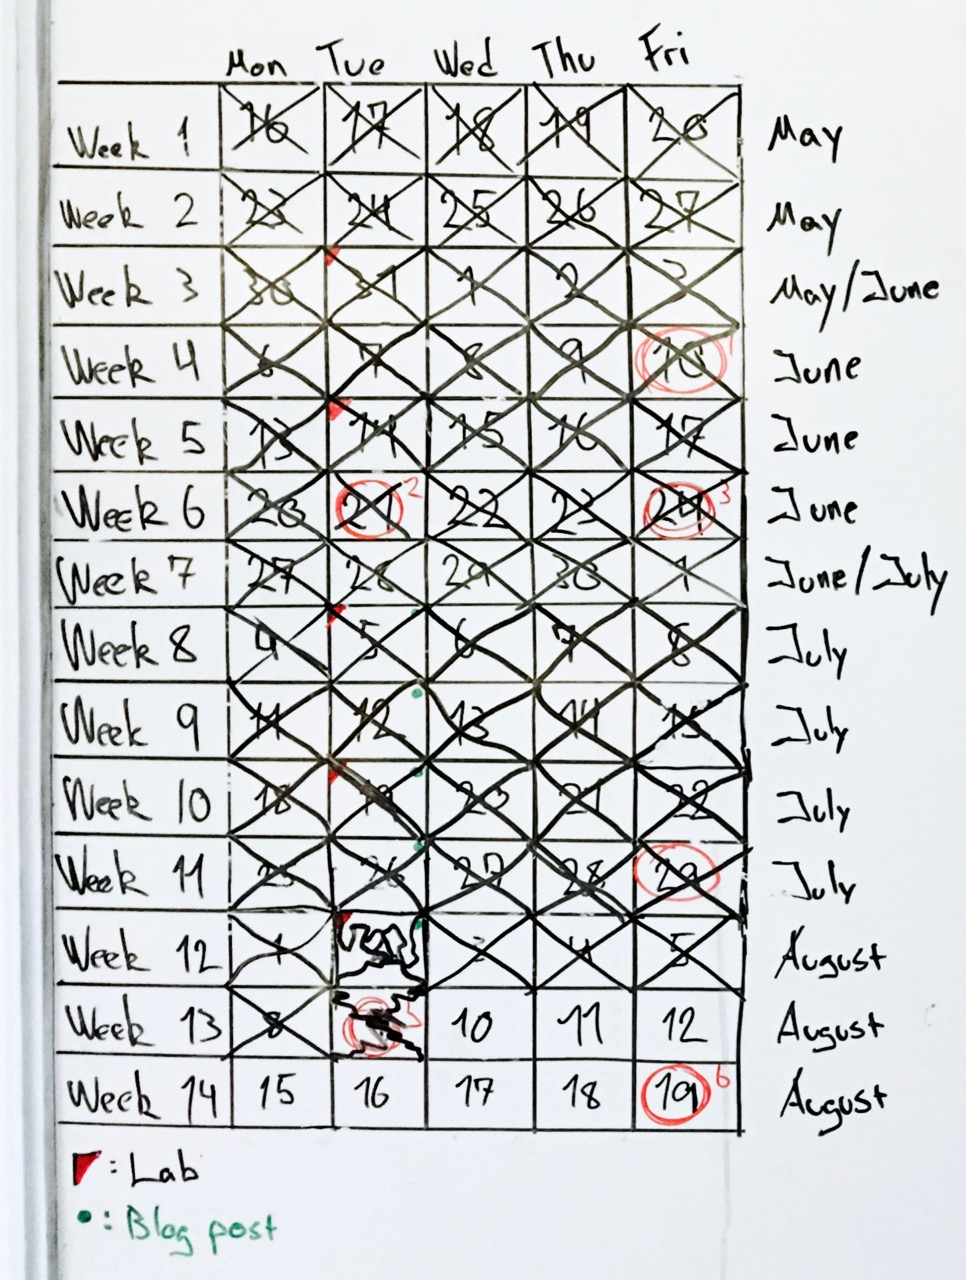
\includegraphics[width=0.35\textwidth]{whiteboard2}
    \caption{Progress was also tracked on a whiteboard}
\end{figure}

For project management the team wanted to keep things light. After reviewing few solutions \cite{ll-blog-week2} we went with ZenHub \cite{zenhub}. It's basically a Chrome extension that hijacks the GitHub repository website and augments it with extra features.

\begin{figure}[H]
    \centering
    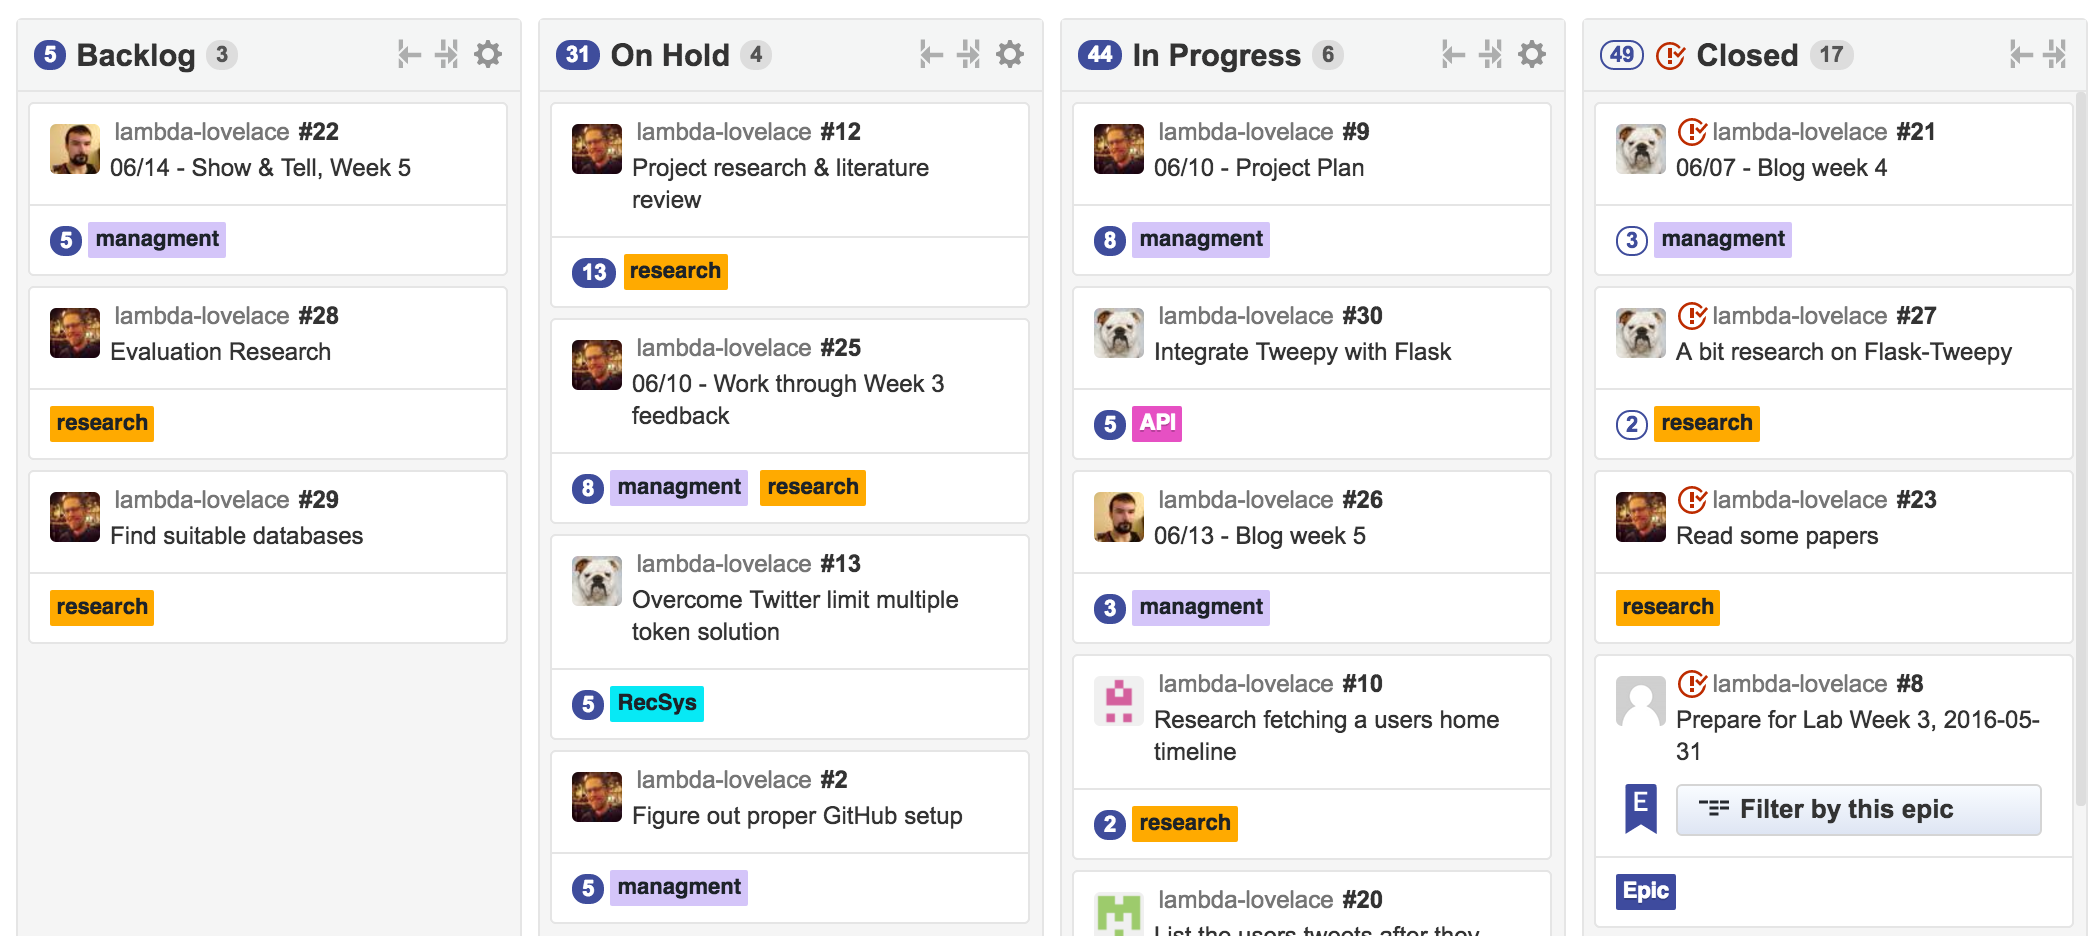
\includegraphics[width=\textwidth]{kanbanboard}
    \caption{ZenHub's Kanban board view of our GitHub issues}
\end{figure}

In the beginning of the project we utilised story points, milestones and burndown charts. However since we met and collaborated closely in person nearly every day we found the management overhead not worth it. Task progress was tracked in about 90 GitHub issues and the Kanban board view gave a good overview.

\subsection{Key Challenges} 

\subsubsection*{Language} 
Tweets can be in many languages. This is a challenge for our recommender system because a stopword in one language might be a legitimate word in another. Hence, the $\lambda$ Lovelace system is geared towards English speaking users.




\subsubsection*{Twitter API rate limits} 

Twitter has imposed rate limits on access to their API. Each form of accessing the API, such as accessing the users home-timeline or their likes, has different rate limits. There is a 15 minute window that the limits apply to. So for a user home-timeline API call, only 15 requests are allowed in a window of 15 minutes or for a search API call only 180 requests every 15 minutes is allowed. To work around this, the project uses a database to store tweets by sending requests during these windows and Celery to automate this process.
    
\subsubsection*{Home timeline limit} 

Only the latest 800 tweets can be requested. This poses a problem for users that follow a lot of accounts, or for users that check Twitter very infrequently. For example, user \textit{Y} who follows twice as many accounts as user \textit{X} will see 800 tweets in half the time that user \textit{X} will. This is the projects primary motivator to periodically collect and cache tweets in the database.




\subsubsection*{Evaluations in iOS client} 
Reusing our Swift code for an iOS evaluation app seemed logical at the time. However distribution hurdles greatly limited our reach. In retrospect going for a JavaScript website with embedded tweets \cite{embed-tweet} might have been better. This was a challenge we were unfortunately not able to overcome due to time constraints.

\subsubsection*{Selection of a document database} 
Storage was an issue for us, as the nature of data from Twitter's API was in a very basic JSON format. Rather than using a relational database, we used the document database RethinkDB to circumvent this issue entirely as RethinkDB is aimed at storing JSON data.

\subsubsection*{Combining recommender system data} 
The need to concretely tie together all factors when recommending tweets was solved by the use of a decimal ranking system. Tweets are weighted according to the various inputs given to the recommender system, then sorted based on the output that results from the input provided.




\subsection{Strengths And Weaknesses} 
The $\lambda$ Lovelace system holds a powerful recommender system that has proven to give users higher quality tweets, based on our experiments. The use of an approach that utilises the users interests was vital to our approach and resulted in the main strength of our system - the quality of recommendations.

However, there are a few weaknesses with the system. For example, if a user likes a tweet for its content, but there are no term frequency document terms in that tweet, the like will have no immediate effect. The like will only come into effect once the user has engaged in enough activity on their personal timeline with that term to place the term into their term frequency document, similar to a "cold start". 



$\lambda$ Lovelace also competes with several other mobile clients for the market share of Twitter users. We could have spent the entirety of this project replicating the functionality of other Twitter clients, but this would not have yielded a system with our niche of recommendation. Despite this, it is still a weakness in the system.


\subsection{Key Contributions} 


$\lambda$ Lovelace takes up a very niche area in the app store. We could not find another iPhone app Twitter client that provides recommendations on tweet themselves. The fact that Twitter itself is attempting recommendations speaks volumes of the importance of recommender systems to the Twitter ecosystem. That there are not more offering for Twitter recommender systems on either the Android or Apple platforms is astounding and lends merit to the novelty of the $\lambda$ Lovelace system. 





\subsection{Future Work} 

\subsubsection*{Search API} 
Tweets from accounts that the user is not following did not make it into the current iteration of the $\lambda$ Lovelace system. We attempted to add this functionality, but did not have the time to filter out obscene/useless tweets. As the recommender system is the main appeal of this project, it was decided to shelve the Search API. Future work would involve placing tweets from the search API (Found through popular term frequency document terms) in the list of recommendations.

\subsubsection*{"Cold Start" For New Terms} 
Adding non-stop-words from the liked tweet to the term frequency document is possible, but this could easily be overkill. Disliking tweets that do not contain terms has little effect however, as these tweets will appear lower in the list of recommendations regardless. Adding non-stop-words from liked tweets that do not have term frequency document terms to the second net functionality would be an ideal solution to this problem. It would not strongly affect the good quality recommendations, but would provide immediate minor results to the user. 



\subsubsection*{iOS App Basic Twitter Functionality} 
In order to enhance user adoption, the iOS app requires the full capabilities (composing tweets, retweeting, following, etc) so that it is not ignored in favour of other apps that already provide this functionality.


\newpage



\section{Appenix}



\subsection{Twitter Intro}
Twitter is a microblogging social network where each post or \textit{tweet} is no more than 140 characters in length. A typical Twitter user \textit{follows} multiple other users (followees) and get followed by other users (followers). By following other users they subscribe to all of their tweets and re-tweets (rebroadcast of other user's tweets). The \textit{timeline} is a chronological feed of those tweets.


\subsection{OAuth login}
\hypertarget{oauth}
OAuth is a popular form of authentication which is used for identifying application's identity and for allowing users to grant applications access permissions. The OAuth protocol does not reveal a user's username nor password to third party applications, making it more secure than traditional authentication schemes.

\subsection{Resources}
Below are summarised lists of the resources we've utilised while working on the project: software, libraries, frameworks, tutorials, etc.








\subsubsection*{Front-End Swift Libraries \& Frameworks}
\begin{itemize*}
    \item \textbf{Swift} \cite{swift}: Programming language developed by Apple
    \item \textbf{iOS} \cite{ios}: Mobile operating system for the Apple iPhone and iPad
    \item \textbf{Alamofire} \cite{alamofire}: Elegant HTTP networking library
    \item \textbf{SwiftyJSON} \cite{swiftyjson}: Easier JSON data handling
    \item \textbf{OAuthSwift} \cite{oauthswift}: Swift based OAuth library for iOS
\end{itemize*}

\subsubsection*{Back-End Python Libraries \& Frameworks}
\begin{itemize*}
    \item \textbf{Flask} \cite{flask}: Micro web development framework for Python
    \item \textbf{Tweepy} \cite{tweepy}: Easy-to-use Python library for accessing the Twitter API
\end{itemize*}

\subsubsection*{Software \& Services}
\begin{itemize*}
     \item \textbf{Git} \cite{git}: Version control software for collaborative software development
     \item \textbf{Github} \cite{github}: Project hosting website that uses Git
     \item \textbf{Facebook Messenger} \cite{messenger}: Social media messaging application
     \item \textbf{Google Drive} \cite{drive}: Online storage system for documents
     \item \textbf{Zenhub} \cite{zenhub}: Chrome browser extension for Github
     \item \textbf{Omnigraffle} \cite{omnigraffle}: Graphics creation wesbite
     \item \textbf{Slack} \cite{slack}: Software-focused messaging app that integrates with Git
     \item \textbf{Pixlr} \cite{pixlr}: Online image editor
     \item \textbf{ShareLaTeX} \cite{sharelatex}: Collaborative LaTeX environment
     \item \textbf{Celery} \cite{celery}: Asynchronous job queuing software
\end{itemize*}

\subsubsection*{Learning Resources}
\begin{itemize*}
    \item \textbf{Python Cookbook} \cite{cookbook}: An intermediate-level Python textbook.
    \item \textbf{Python 3 Essential Training} \cite{lynda}: A Lynda.com online training course.
\end{itemize*}

\newpage

\subsection{Evaluation Experiment Flier} \label{full-size-poster}
\begin{figure}[H]
    \centering
    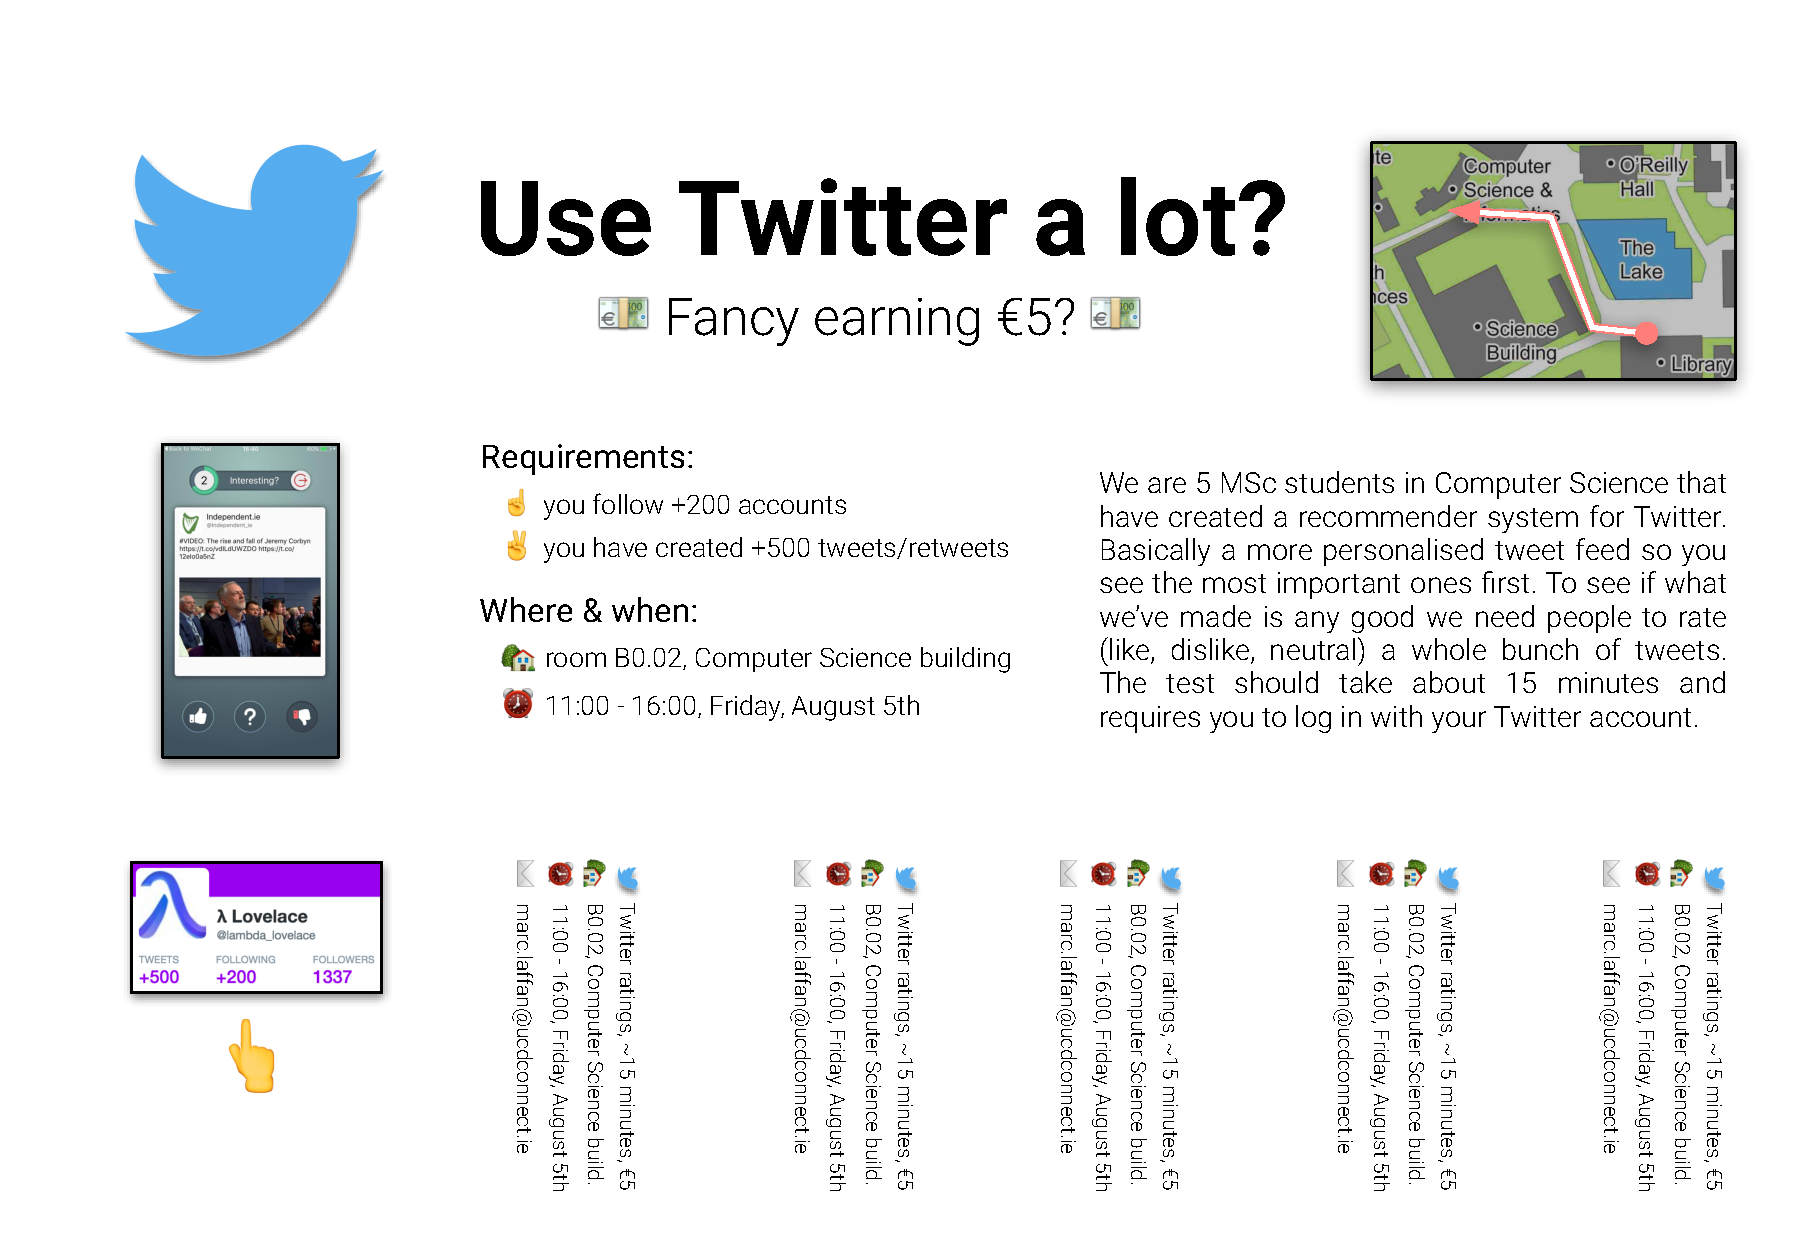
\includegraphics[width=1.5\textwidth,angle=90,origin=c]{evaluation_poster}
\end{figure}


\newpage








\begin{thebibliography}{9} 

\bibitem {information_overload}
    Manuel Gomez-Rodriguez, Krishna Gummadi, and Bernhard Schoelkopf. Quantifying Information Overload in Social Media and its Impact on Social Contagions. In \textit{ICWSM}, 2014.
    
\bibitem {paper1}
    Marcelo G. Armentano and Daniela Godoy and Analía Am. Towards a Followee Recommender System for Information Seeking Users in Twitter.  In \textit{Proceedings of the Workshop on Semantic Adaptive Social Web (SASWeb 2011)}. CEUR Workshop Proceedings, volume 730, pages 27–38, 2011.
    
\bibitem {paper2}
    J. Hannon, M. Bennett, and B. Smyth. Recommending twitter users to follow using content and collaborative filtering approaches. In \textit{Proceedings of the fourth ACM conference on Recommender systems}, pages 199–206. ACM, 2010.
    
\bibitem {paper3}
    O. Phelan, K. McCarthy, and B. Smyth. Using Twitter to recommend real-time topical news. In \textit{Proceedings of the third ACM Conference on Recommender Systems}, pages 385–388. ACM, 2009.
    
\bibitem {gitrepo}
	$\lambda$ Lovelace main code repository on GitHub \\
	\url{https://github.com/jonrh/lambda-lovelace/}
	
\bibitem {ucdgithub}
	Negotiated Learning Project organisation on GitHub \\
	\url{https://github.com/ucd-nlmsc-teamproject}
	
\bibitem {ll-blog}
	$\lambda$ Lovelace blog, \url{https://jonrh.github.io/lambda-lovelace/}
	
\bibitem {ll-blog-week2}
	$\lambda$ Lovelace blog, Week 2: Project Managment Tool Selection \\ \url{https://goo.gl/mjw4M2}
	
\bibitem {ll-blog-week9}
	$\lambda$ Lovelace blog, Week 9: DB, Docker, CI/CD \\ 
	\url{https://goo.gl/HzoLH7}
	
\bibitem {ll-blog-week10}
	$\lambda$ Lovelace blog, Week 10: Caching Data \\ 
	\url{https://goo.gl/8f6eLV}
	
\bibitem {ll-blog-week11}
	$\lambda$ Lovelace blog, Week 11: Recommender System \& CD \\ 
	\phantom{ } \url{https://goo.gl/DbxIBI}
	
\bibitem {twitter-opt-in}
    Twitter blog post: \textit{Never miss important Tweets from people you follow} \\
    \phantom{ } \url{https://goo.gl/UqTIRz}

\bibitem {clark1}
    Andrew Clark Tweet One \\
    \phantom{ } \url{https://twitter.com/acdlite/status/745345694949507072}
    
\bibitem {clark2}
    Andrew Clark Tweet Two \\
    \phantom{ } \url{https://twitter.com/acdlite/status/745273848233230337}
	
\bibitem {swift}
	Swift official website \url{https://developer.apple.com/swift/}
	
\bibitem {ios}
	iOS official website \url{http://www.apple.com/ie/ios/}
	
\bibitem {zenhub}
	ZenHub, \url{https://www.zenhub.com/}

\bibitem {flask}
    Flask, \url{http://flask.pocoo.org/}
    
\bibitem {git}
    Git, \url{https://git-scm.com/}

\bibitem {github}
    GitHub, \url{https://github.com/}

\bibitem {messenger}
    Facebook Messenger \url{https://www.messenger.com/}

\bibitem {drive}
    Google Drive, \url{https://www.google.ie/drive/}

\bibitem {omnigraffle}
    Omnigraffle, \url{https://www.omnigroup.com/omnigraffle}

\bibitem {slack}
    Slack, \url{https://slack.com/}
    
\bibitem {pixlr}
    Pixlr, \url{https://pixlr.com/}
     
\bibitem {sharelatex}
    ShareLaTeX, \url{https://www.sharelatex.com}
    
\bibitem {celery}
    Celery, \url{http://www.celeryproject.org/}

\bibitem {Swift}
    Swift, \url{https://developer.apple.com/swift/}
    
\bibitem {oauthswift}
    OAuthSwift GitHub repository \\
    \phantom{ } \url{https://github.com/OAuthSwift/OAuthSwift}
    
\bibitem {alamofire}
    Alamofire GitHub repository \\
    \phantom{ } \url{https://github.com/Alamofire/Alamofire}
    
\bibitem {swiftyjson}
    SwiftyJSON GitHub repository \\
    \phantom{ } \url{https://github.com/SwiftyJSON/SwiftyJSON}
    
\bibitem {django}
    Django, \url{https://www.djangoproject.com/}
    
\bibitem {bottle}
    Bottle, \url{http://bottlepy.org/docs/dev/index.html}
    
\bibitem {tweepy}
    Tweepy GitHub repository \url{https://github.com/tweepy/tweepy}

\bibitem{twitter-rest-api}
    Twitter REST API \\
    \phantom{ } \url{https://dev.twitter.com/rest/public}

\bibitem {streaming}
    Twitter Streaming API \\ 
    \phantom{ } \url{https://dev.twitter.com/streaming/userstreams}
    
\bibitem {ceo}
    Cio.com, Twitter's Challenge: Personalization, Co-Founder Says \\
    \phantom{ } \url{http://goo.gl/gt2fSs}

\bibitem {embed-tweet}
    Twitter API Documenation, Embed a Single Tweet in a Webpage \\
    \phantom{ } \url{https://dev.twitter.com/web/embedded-tweets}
    
\bibitem {max}
    Twitter Developers Forums, \textit{Max user streams per application?} \\
    \phantom{ } \url{https://goo.gl/YnYuL8}
    
\bibitem {cursor}
    Tweepy Cursor Tutorial \\ 
    \phantom{ } \url{http://tweepy.readthedocs.io/en/v3.5.0/cursor_tutorial.html}

\bibitem {couchbase}
    Couchbase, \url{http://www.couchbase.com/}
    
\bibitem {rethinkdb}
    RethinkDB, \url{http://rethinkdb.com/}

\bibitem {couchdb}
    CouchDB, \url{http://couchdb.apache.org/}

\bibitem {mongodb}
    MongoDB, \url{https://www.mongodb.com/}

\bibitem {elasticsearch}
    ElasticSearch \url{https://www.elastic.co/products/elasticsearch}
    
\bibitem {cookbook}
    Python Cookbook \\
    \phantom{ } \url{http://shop.oreilly.com/product/0636920027072.do}
    
\bibitem {lynda}
    Python 3 Essential Training \\
    \phantom{ } \url{https://goo.gl/lrz4eT}
    
\bibitem {hockeyapp}
    HockeyApp, \url{https://hockeyapp.net/}
    
\bibitem {heroku}
    Heroku, \url{https://www.heroku.com/}
    
\bibitem {circleci}
    CircleCI, \url{https://circleci.com/}
    
\bibitem {distelli}
    Distelli, \url{https://www.distelli.com/}
    
\bibitem {dockercloud}
    DockerCloud, \url{https://cloud.docker.com/}
    
\bibitem {jenkins}
    Jenkins, \url{https://jenkins.io/}


\end{thebibliography}


\newpage

\end{document}